% Build with: latexmk -lualatex -interaction=nonstopmode -halt-on-error MathStep.tex
% Self-contained source. No external bibliography, images, or font files required.
\documentclass[11pt,a4paper]{article}
\usepackage[margin=25mm,headheight=15pt]{geometry}
\usepackage{fontspec}
\setmainfont{Linux Libertine O}
\setsansfont{Lato}
\setmonofont{DejaVu Sans Mono}[Scale=0.80]
\usepackage{amsmath,amsthm,mathtools}
\usepackage{unicode-math}
\setmathfont{latinmodern-math.otf}
\usepackage{microtype}
\usepackage{booktabs,longtable,tabularx,array}
\usepackage[table]{xcolor}
\definecolor{ink}{HTML}{253538}
\definecolor{accent}{HTML}{53624B}
\definecolor{light}{HTML}{F2F4ED}
\definecolor{rulegray}{HTML}{C6CDBF}
\usepackage{enumitem}
\setlist{nosep,leftmargin=1.6em}
\usepackage{fvextra}
\DefineVerbatimEnvironment{code}{Verbatim}{fontsize=\small,breaklines=true,breakanywhere=false,frame=leftline,framesep=3mm,rulecolor=\color{rulegray},xleftmargin=3mm,tabsize=2}
\usepackage{tikz}
\usetikzlibrary{arrows.meta,positioning,fit}
\usepackage{fancyhdr}
\usepackage{titlesec}
\usepackage{needspace}
\usepackage{etoolbox}
\pretocmd{\section}{\Needspace{10\baselineskip}}{}{}
\pretocmd{\subsection}{\Needspace{5\baselineskip}}{}{}
\clubpenalty=10000
\widowpenalty=10000
\raggedbottom
\usepackage{hyperref}
\hypersetup{bookmarksdepth=2,colorlinks=true,linkcolor=accent,citecolor=accent,urlcolor=accent,pdftitle={MathStep: A Proof Language of Mathematical Steps},pdfauthor={OpenAI},pdfsubject={A technical language-design study grounded in ProveIt and Leant}}
\usepackage{xurl}
\urlstyle{same}
\pagestyle{fancy}
\fancyhf{}
\fancyhead[L]{\sffamily\small MathStep / Technical design study}
\fancyhead[R]{\sffamily\small\thepage}
\renewcommand{\headrulewidth}{0.3pt}
\titleformat{\section}{\sffamily\Large\bfseries\color{ink}}{\thesection}{0.7em}{}
\titleformat{\subsection}{\sffamily\large\bfseries\color{ink}}{\thesubsection}{0.6em}{}
\titleformat{\subsubsection}{\sffamily\normalsize\bfseries\color{ink}}{\thesubsubsection}{0.6em}{}
\titlespacing*{\section}{0pt}{3.0ex plus .7ex}{1.2ex}
\titlespacing*{\subsection}{0pt}{2.2ex plus .5ex}{.8ex}
\setlength{\parindent}{0pt}
\setlength{\parskip}{.6em}
\setlength{\emergencystretch}{2.5em}
\setcounter{tocdepth}{1}
\newtheorem{proposition}{Proposition}[section]
\newtheorem{definition}[proposition]{Definition}
\newtheorem{principle}[proposition]{Design principle}
\theoremstyle{remark}
\newtheorem{remark}[proposition]{Remark}
\newcommand{\ms}{\textsc{MathStep}}
\newcommand{\ty}[1]{\texttt{#1}}
\newcommand{\R}{\mathbb{R}}
\newcommand{\N}{\mathbb{N}}
\newcommand{\C}{\mathbb{C}}
\newcommand{\Deps}{\operatorname{Deps}}
\newcommand{\Ax}{\operatorname{Ax}}
\newcommand{\FV}{\operatorname{FV}}
\newcommand{\pv}{24ce8bd743eaab64a91ce90725ea00f498d319d2}
\newcommand{\lv}{c36adf114035fb2fba6c276b63944cc613b31668}
\newcommand{\source}[1]{\par{\small\textit{Repository evidence:} #1}\par}
\newcommand{\designnote}[1]{\par\smallskip\noindent\colorbox{light}{\parbox{\dimexpr\linewidth-2\fboxsep\relax}{\textbf{Design status.} #1}}\par\smallskip}
\newcolumntype{Y}{>{\raggedright\arraybackslash}X}
\newcolumntype{L}[1]{>{\raggedright\arraybackslash}p{#1}}
\begin{document}
\hypersetup{pageanchor=false}
\begin{titlepage}
\color{ink}
\vspace*{13mm}
{\sffamily\small\color{accent} PROOF LANGUAGES / ELABORATION / VERIFIED SYNTHESIS\par}
\vspace{12mm}
{\sffamily\fontsize{33}{39}\selectfont\bfseries MathStep\par}
\vspace{4mm}
{\sffamily\fontsize{23}{29}\selectfont A Proof Language of\par Mathematical Steps\par}
\vspace{9mm}
{\Large A design grounded in ProveIt and Leant\par}
\vspace{12mm}
\par\noindent\rule{\linewidth}{0.5pt}\par
\vspace{4mm}
{\large\textbf{The central proposal}\par}
The author writes the mathematical decisions and intermediate claims. A scoped, method-directed elaborator reconstructs routine details. The resulting proof is checked against an independently fixed statement, with explicit assumptions and reproducible certificates.
\vspace{5mm}
\par\noindent\rule{\linewidth}{0.5pt}\par
\vfill
{\sffamily Prepared for Vladimir Reshetnikov\par}
{\sffamily 5 September 2026\par}
\vspace{5mm}
{\small A technical concept and implementation plan, not a claim of an implemented language. The repository case studies are source reviews; the proposed syntax and reconstructed examples have not been compiled as a new language.}
\end{titlepage}
\hypersetup{pageanchor=true}

\begin{abstract}
A useful mathematical proof is not a transcript of every operation needed to construct a term in dependent type theory. It is a structured account of the choices that make the argument work: the induction invariant, the right substitution, the relevant branch, the neighborhood on which an identity holds, or the lemma that reduces the problem. Much of the remaining formal text is reconstructible bookkeeping. But some apparently routine details are indispensable hypotheses, and hiding them carelessly changes the theorem.

This article proposes \ms, a proof language whose primary unit is a typed mathematical step rather than an individual tactic invocation. The design is grounded in four inspected ProveIt modules and in Leant's existing synthesis, translation, verification, and provenance boundaries. Worked examples cover differentiation of an algebraic branch, branch uniqueness, differentiation of identities on open sets, reflected dyadic indices and finite-sum substitution, and structural induction on formal derivations. The proposal combines declarative assertions, domain-specific methods with explicit proof obligations, a scoped obligation ledger, bounded synthesis, and frozen proof capsules. It specifies the relationship between source meaning, elaboration, kernel checking, axiom policy, and explanatory structure; gives a small core semantics and a conditional soundness argument; and develops a concrete Lean-hosted implementation and evaluation plan. Concision is treated as reduced authoring and maintenance effort, not as a contest to replace every proof by a single opaque command.
\end{abstract}

\section*{Scope and evidence}
\addcontentsline{toc}{section}{Scope and evidence}
The ProveIt examples were inspected at commit
\begin{center}\small\texttt{\pv}\end{center}
and Leant at
\begin{center}\small\texttt{\lv}.\end{center}
The inspected ProveIt toolchain file selects Lean \ty{v4.32.0}. The bibliography links to immutable source revisions where repository evidence matters. Public documentation was consulted on 5 September 2026; references to its current version explain architecture rather than certify API compatibility with the pinned project.\cite{proveit-toolchain,lean-elaboration}

The sample consists of four source files, selected to expose different forms of proof friction. It is not a statistical survey of ProveIt, an audit of all its results, or a measurement of Leant's present success rate. Statements about current behavior are separated from design recommendations. No end-to-end Lean build or synthesis benchmark was run for this article. Mathematical transformations in the case studies are justified explicitly, but all \ms\ programs are proposed syntax. Shared library development is counted as a real cost, not hidden behind short examples.

\newpage
\begingroup
\setlength{\parskip}{0pt}
\small
\tableofcontents
\endgroup
\newpage

\section{What should become shorter?}\label{sec:problem}

\subsection{The object to compress is an argument, not merely text}
Suppose a mathematician says, ``Differentiate the induction hypothesis and use the chain rule.'' This sentence contains several kinds of information. It selects a strategy, identifies a previously established identity, and invokes a known mathematical transformation. It leaves implicit the introduction of a point, the conversion of equality on an open set into equality near that point, the construction of derivative certificates, and the transport of an equality between differently written expressions.

A proof language can improve this interaction in two fundamentally different ways. It can abbreviate an existing tactic script, or it can make the mathematical operation itself a first-class construct with a precisely specified elaboration. The second is the more interesting opportunity. The user should not need to remember which combination of a filter lemma, a derivative congruence lemma, and a composition theorem implements the familiar mathematical operation.

However, the sentence is not valid in every context. Equality at one point does not imply equality of derivatives there. A system that silently overlooks this distinction is not improving formalization; it is discarding mathematical content. The right objective is therefore:
\begin{quote}
Preserve the choices that determine the argument, reconstruct the consequences that are routine in a declared mathematical context, and expose any unmet condition that makes the intended step invalid.
\end{quote}
This is a design objective, not a psychological claim that all mathematicians think in the same language. A finished proof normally presents a reconstructed argument, not the false starts and experiments by which its author discovered it.

\subsection{Four sources of verbosity}
The inspected proofs suggest a useful classification.

\textbf{Representational friction} comes from coercions, projections, explicit arguments, binder bookkeeping, and conversion between pointwise and function-level formulations. These details matter to the type checker, but often do not deserve equal visual weight with the proof idea.

\textbf{Library-interface friction} comes from locating a theorem, knowing the orientation and order of its parameters, and adapting its conclusion to the present goal. A long theorem name may be an excellent global identifier while being a poor unit of mathematical prose.

\textbf{Routine derivation} includes linear inequalities from current bounds, polynomial normalization, construction of conjunctions, and rebuilding an inductive constructor from induction hypotheses. These are genuine proofs, but they can often be generated within a small, predictable search space.

\textbf{Essential mathematical content} includes a branch condition, an induction motive, a convergence hypothesis, or the domain on which a function identity is valid. Such information should become easier to express and inspect, not easier to omit accidentally.

The categories depend on the audience and context. A cast identity can be the central point of a theorem about truncated subtraction. A branch condition that is automatic in one section may be a new hypothesis in another. Consequently, \ms\ does not globally decree that particular classes of facts are uninteresting. It controls their default presentation and reconstruction through explicit local profiles.

\subsection{The shortest proof need not be the best proof}
Replacing an entire argument by \ty{by search} may reduce visible characters while increasing uncertainty, search cost, and repair effort. Conversely, a two-line calculation may be better than a one-line invocation of a large theorem because the calculation makes the mechanism visible.

The proposed optimization target is multi-dimensional:
\[
\mathcal{C}=\bigl(C_{\mathrm{author}},C_{\mathrm{reader}},C_{\mathrm{repair}},
C_{\mathrm{search}},C_{\mathrm{check}},C_{\mathrm{library}}\bigr).
\]
These components represent author effort, reader effort, maintenance effort, discovery cost, replay cost, and the cost of the supporting mathematical vocabulary. There is no reason to collapse them immediately into one universal score. In particular, an implementation should not advertise a large source reduction without accounting for new methods, support lemmas, and cached proof artifacts.

\subsection{Do not make Lean a straw man}
Lean already separates elaboration from kernel checking and supports structured proofs, calculations, extensible syntax, and automation. Its tactic proofs are elaborated into proof terms.\cite{lean-elaboration,lean-tactics} Thus the proposal is not that rigor currently requires a user to write every inference by hand. It is that the \emph{default unit of interaction} can better match a mathematical step, and that the relationship among omitted detail, method contracts, explanations, and replay can become systematic.

A fair comparison must include expert-written Lean using the same mathematical lemmas and automation. Some of the examples below may admit excellent short Lean proofs already. That would be evidence for useful components of the proposed implementation, not a refutation of the larger interface design.

\section{What the repository examples reveal}\label{sec:evidence}

\subsection{A compact map of the inspected material}
\begin{longtable}{@{}L{.23\linewidth}L{.34\linewidth}L{.37\linewidth}@{}}
\toprule
Module & Mathematical step & Detail that must remain accountable\\
\midrule
\endhead
\ty{AlgebraicInverse-}\newline\ty{GermAnalytic.lean} & Differentiate an explicit root; identify the correct quadratic branch. & Nonvanishing radicand at the differentiation point; sign of the selected branch.\\[4pt]
\ty{Autonomous-}\newline\ty{IteratedDeriv.lean} & Differentiate an inductive identity on an open set. & Neighborhood equality, correct induction scope, derivative assumptions only on the necessary range.\\[4pt]
\ty{AliasQBinomial-}\newline\ty{Bridge.lean} & Reflect a dyadic index and substitute a sample formula under a sum. & Natural subtraction bounds, nonzero denominator, local index membership, real/complex coercions.\\[4pt]
\ty{NaturalDeduction/}\newline\ty{Calculus.lean} & Map derivations along an inclusion of axiom schemas. & Every constructor case, contextual indices, and the distinction between object logic and metalogic.\\
\bottomrule
\end{longtable}
The first three files are in the FabiusFunction development; the fourth is in the propositional natural-deduction development. Their source is the basis of Sections~\ref{sec:root}--\ref{sec:structural}.\cite{proveit-root,proveit-ode,proveit-alias,proveit-nd}

\subsection{A representative low-level fragment}
The following excerpt from the autonomous-derivative proof is particularly instructive. Its line wrapping is adjusted for the page:
\Needspace{82pt}
\begin{code}
rw [heq.deriv_eq]
have hcomp : HasDerivAt (G n ∘ W)
    (G' n (W x) * φ (W x)) x :=
  (hGd n x hx).comp x (hW x hx)
rw [hcomp.deriv, hGs n x hx]
\end{code}
Immediately before this excerpt, the source establishes \ty{heq}, the filter equality
\[
\operatorname{iteratedDeriv}(n,W)=^{\!\mathrm{ev}}_{\mathcal{N}(x)}G_n\circ W,
\]
constructed using \ty{Filter.eventuallyEq\_of\_mem} and the neighborhood supplied by openness.\cite{proveit-ode}

The source explicitly solves a real mathematical problem: the induction hypothesis is restricted to a set, while differentiation is a local operation. A useful higher-level construct should package this reasoning, not delete it. The method's result must include precisely the congruence and chain-rule evidence that the existing proof constructs.

\subsection{A second example: a long name is not a long argument}
The dyadic bridge calls a theorem named
\Needspace{46pt}
\begin{code}
fabiusFunction_dyadic_eq_
  qBinomialThueMorseDyadicTranslatedFormulaIn_real
\end{code}
where the line break is editorial. The source then adapts a reflected natural-number index and casts the result into a complex-valued sum.\cite{proveit-alias} The mathematics is a substitution of one exact sample formula into another identity. The global name remains useful for precise identification; a local mathematical vocabulary should allow the proof to say \ty{dyadic sample formula} while recording which constant, instantiation, and domain conditions that phrase denotes.

This suggests a separation between \emph{reader-facing names} and \emph{certificate identity}. Aliases should be lexical and versioned. They should never mean ``whatever a search engine currently thinks this phrase refers to.''

\section{A language of checked mathematical steps}\label{sec:concept}

\subsection{The basic contract}
A \ms\ proof is a sequence or tree of assertions, reductions, choices, and structured subproofs. A step contains enough information to determine what is being claimed and enough guidance to make reconstruction tractable. It does not have to contain the entire reconstruction.

The design has three contracts.

\textbf{Meaning.} The formal statement, binder scopes, types, notation, and relevant instances are fixed independently of whether proof search succeeds. Search is not allowed to reinterpret an ambiguous assertion as whichever proposition happens to be provable.

\textbf{Evidence.} Every accepted assertion has a proof of that exact formal statement in the declared context. Methods, learned models, external provers, and synthesis engines propose evidence; they do not add axioms or pronounce a theorem true.

\textbf{Reconstruction.} The accepted interpretation and evidence are retained in a stable form. Rechecking a finished proof does not require rediscovering the same argument, contacting a model, or winning a race among competing tactics.

These contracts are independent. A kernel-accepted proof of a misinterpreted statement satisfies the second but not the first. A readable proof that relies on an unstable search process may satisfy the first two but fail the third.

\subsection{A small language first, not unrestricted English}
The first implementation should retain Lean's expression language and type elaborator. It should add a small declarative proof layer, rather than attempt a new foundation, a new mathematical library, and a free-form English parser simultaneously.

The surface could eventually have two presentations: a concise symbolic notation and a controlled prose notation. Both must elaborate to the same typed intermediate representation. Arbitrary explanatory prose can coexist with the proof but has no logical force. A natural-language assistant may propose a formal step; accepting that step commits to its displayed formal interpretation, not to an invisible model interpretation.

\designnote{All code blocks headed by mathematical prose in the following sections describe proposed syntax. Lean expressions inside them are illustrative. They are not claims that these keywords or domain methods are currently implemented.}

A typical block might read:
\Needspace{106pt}
\begin{code}
proof
  take x in U
  have local_identity : D[n] W = G[n] o W near x
    from induction_hypothesis, U_open
  differentiate local_identity at x
    using W_equation, G_derivative
  conclude by recurrence
\end{code}
The phrase \ty{near x} denotes a specific neighborhood-filter relation, not an informal modifier. The method \ty{differentiate} carries a typed contract. An implementation may present this block more compactly once the reader knows the vocabulary, but the expandable structured version should always remain available.

\subsection{Assertions are the durable interface}
An imperative proof records how to transform one proof state into the next. A declarative step records an assertion that can survive many changes to its reconstruction. \ms\ deliberately makes assertions the durable interface between the human document and automation.

For example:
\Needspace{46pt}
\begin{code}
have square : (8*z + 1)^2 = 1 + (64/9)*q
  from equation by algebra
\end{code}
The assertion remains intelligible if the implementation switches from ring normalization to a linear-combination certificate. Conversely, a change in the assertion is a meaningful mathematical change and deserves review even when the resulting theorem still checks.

It follows that a proof document has two related dependency graphs: the graph of \emph{assertions chosen by the author}, and the finer graph of \emph{evidence used to justify them}. The second can be hidden by default. The first should not be erased merely because an automated prover found a shorter path to the final theorem.

\section{Surface language and scope discipline}\label{sec:surface}

\subsection{A minimal set of constructs}
The core need not contain a large inventory of special phrases. The following forms cover the stable logical structure:
\Needspace{142pt}
\begin{code}
take x : A                       -- universal introduction
assume h : P                     -- implication introduction
let y := t                       -- a local definition
have h : P by method             -- a checked local assertion
choose x with hx : P x from e    -- existential elimination
suffices h : Q by continuation   -- reduction to an intermediate goal
calc ...                         -- typed relational composition
cases e with ...                 -- elimination with named branches
induct n generalizing x with ... -- an explicit induction choice
show P by method                 -- close the current goal
\end{code}
These forms are intentionally familiar. The design difference is not the novelty of individual keywords. It is that each step participates in a common obligation, synthesis, explanation, and replay protocol.

A theorem's declaration supplies an expected proposition. \ty{take} and \ty{assume} must match its binder structure or an explicitly selected subgoal. A new arbitrary assumption is not silently added to make a proof go through. A \ty{have} adds a fact only after its proof is checked; it may be edited with a temporary hole in an exploratory document, but a hole cannot appear in an accepted export.

\subsection{Elaborate meaning before searching for evidence}
Consider \ty{x / y}. Its meaning depends on the types of \ty{x} and \ty{y}, the selected division operation, and any coercions. A proof of a statement over rational numbers is not automatically a proof of a visually similar statement about natural-number division. Similarly, a custom notation can change what a familiar mathematical symbol denotes.

For this reason, theorem statements should be elaborated under a pinned declaration context before proof-producing services run. At every step, the user can inspect a ``fully typed'' view: resolved constant names, inserted coercions, local instance arguments, universe parameters, and the precise proposition. Ordinary type inference remains useful; proof-success-driven choice between materially different statements does not.

Some elaboration constraints genuinely depend on a supplied witness, especially in dependent mathematics. The restriction is not that all elaboration must be globally complete before any subterm is built. It is that the user-facing assertion's meaning must not be silently selected by unrestricted proof search. Where a witness determines an index, the source must expose the dependency, and finalization must show the resolved proposition before sealing it.

\subsection{A ledger of obligations, not a bag of assumptions}
Each method creates an obligation ledger. An entry contains a proposition, a local telescope, an origin in the source, a mathematical role, and an eventual proof. For example, cancelling a denominator can create:
\Needspace{82pt}
\begin{code}
obligation 17
  role: denominator is nonzero
  context: n : Nat
  claim: (2 : Real)^n != 0
  origin: dyadic-index normalization
\end{code}
A positivity procedure can discharge this automatically. An unresolved entry remains a visible failure attached to the original step. It is never promoted to an assumption.

The ledger is scoped. A fact proved under \ty{0 < x} may be used inside that branch, not in a sibling branch. A fact about an arbitrary \ty{k} in a finite set carries that membership assumption. A temporary definition retains its defining value and type. ``Automatic'' means automatic production and checking of evidence, not deletion of a premise.

Obligations also need scheduling. A method may first need a cast bound to normalize an expression and then use the normalized expression to close an algebraic goal. Dependencies between such entries form a directed graph. The scheduler should detect a cycle in which each missing side condition is justified only by the other, rather than presenting two mutually reassuring green markers.

\subsection{Local context is not global proof-search permission}
A large file may make thousands of declarations available. That does not mean every routine step should search all of them. A profile supplies a bounded mathematical vocabulary and a search policy. Local facts are indexed by type and scope; expensive theorem search is an explicit action.

The distinction between guidance and restriction should be visible:
\Needspace{46pt}
\begin{code}
have P from h1, h2 by algebra
have P using only h1, h2 with real_ring by algebra
\end{code}
In the first form the listed facts guide reconstruction. In the second they are the only user-level premise roots permitted, together with the declared method library and its dependency closure. ``Only'' does not ban the logical constants needed to construct a proof; it constrains which mathematical assumptions and library packages may support it.

Actual semantic dependence is subtle. A proof term can mention an irrelevant hypothesis without needing it, and two extensionally equal proofs can have different syntactic dependencies. Thus the initial implementation should promise a \emph{conservative dependency audit}, not a decision procedure for mathematically minimal premises. When an intermediate argument is essential to the explanation, the author should write that assertion as a separate step rather than rely on a vaguely enforceable instruction to ``use'' a theorem.

\subsection{Witnesses expose the limits of type-only synthesis}
A term of type $A\to A\to A$ may return either argument. Type correctness alone does not specify the desired computation. The same problem appears when a proof needs a carefully chosen parameter rather than merely an inhabitant of some broad type.

A witness request should therefore state the property that matters:
\Needspace{58pt}
\begin{code}
choose delta > 0 such that
  forall x, abs (x-a) < delta -> abs (f x-f a) < epsilon
by synthesize within continuity_context
\end{code}
The expected result is a witness together with a proof of its property. If \ty{epsilon} is in the current scope, the witness may depend on it. Moving the choice outside that scope changes $\forall\varepsilon\,\exists\delta$ into $\exists\delta\,\forall\varepsilon$, which is not a formatting choice. The elaborator must track such dependencies explicitly.

A distinction is also required between using an existential witness in a proposition and extracting computational data from it. Proposition-level existential elimination, dependent pairs, and noncomputable classical choice have different typing and computational consequences. The language must not conceal this difference behind an undifferentiated \ty{choose}. Its elaborated view should show which operation was used and which logical policy allowed it.

\section{Case study I: an algebraic branch}\label{sec:root}

\subsection{The original mathematical statements}
The inspected file defines
\begin{equation}\label{eq:rootdef}
 R(q)=\frac{\sqrt{1+\frac{64}{9}q}-1}{8},\qquad q\in\R,
\end{equation}
under the Lean name \ty{dyadicRootFun}. Among its results are
\begin{align}
 q\geq0&\implies R(q)+4R(q)^2=\frac49q,\label{eq:rootsolves}\\
 q\geq0,\quad z+4z^2=\frac49q,\quad z> -\frac18
 &\implies z=R(q),\label{eq:rootunique}\\
 R'(0)&=\frac49.\label{eq:rootderiv}
\end{align}
The last assertion is formalized as a \ty{HasDerivAt} statement, not merely an equality involving a total derivative operator. The source builds the derivative of the affine radicand, applies the square-root derivative, composes, simplifies the derivative value, and then accounts for subtraction and division.\cite{proveit-root}

\subsection{A method-directed proof of the defining equation}
A possible source proof is:
\Needspace{106pt}
\begin{code}
theorem root_solves (q : Real) (hq : 0 <= q) :
  R q + 4 * (R q)^2 = (4/9)*q
proof
  let a := 1 + (64/9)*q
  have ha : 0 <= a from hq by order
  have hs : (sqrt a)^2 = a by square_root using ha
  show thesis by algebra using hs unfolding R, a
\end{code}
Here \ty{thesis} is the fixed current target, not a new proposition inferred from the proof. The profile fixes \ty{sqrt} to the real square-root function. The aliases \ty{R} and \ty{a} have explicit definitions. The methods \ty{order}, \ty{square\_root}, and \ty{algebra} are named reconstruction strategies with separate roles.

The actual algebra is short enough to display:
\[
\frac{\sqrt a-1}{8}+4\left(\frac{\sqrt a-1}{8}\right)^2
 =\frac{a-1}{16}
 =\frac49q.
\]
The first equality uses $(\sqrt a)^2=a$ and rational arithmetic. Algebraic normalization alone does not know that square-root identity; it must receive the checked fact or trigger an explicitly registered square-root method that generates its nonnegativity obligation.

A more concise presentation could compress the middle two lines to
\Needspace{34pt}
\begin{code}
show thesis by algebra with real_square_roots
\end{code}
but this is justified only if the expandable evidence shows both the nonnegative-radicand proof and the square-root theorem. The long form may remain preferable for a reader learning the argument.

\subsection{Branch uniqueness: compressing the idea rather than the script}
The source proves uniqueness by factoring the quadratic equation and excluding the unwanted factor with a positivity argument.\cite{proveit-root} A mathematically equivalent, but genuinely different, presentation is:
\Needspace{154pt}
\begin{code}
theorem root_unique (q z : Real)
  (hq : 0 <= q)
  (equation : z + 4*z^2 = (4/9)*q)
  (branch : -1/8 < z) : z = R q
proof
  have square : (8*z + 1)^2 = 1 + (64/9)*q
    from equation by algebra
  have positive : 0 < 8*z + 1 from branch by order
  have identify : 8*z + 1 = sqrt (1 + (64/9)*q)
    from square, positive by positive_square_root
  show thesis from identify by algebra unfolding R
\end{code}
The transformation is valid because multiplying the original equation by $16$ gives
\[
64z^2+16z=\frac{64}{9}q,
\]
so adding $1$ gives the displayed square identity. The branch condition gives $8z+1>0$. For a nonnegative number $u$, the identity $u^2=a$ implies $u=\sqrt a$. Applying this with $u=8z+1$ and rearranging proves~\eqref{eq:rootunique}.

This proof does not actually need \ty{hq} once \ty{square} and \ty{positive} are known: the square identity itself implies the radicand is nonnegative. Keeping \ty{hq} preserves the original theorem's interface; a separate generalization could remove it and be proved explicitly. This small observation illustrates why the system should distinguish ``the same theorem with a different proof'' from ``a strengthened theorem.'' Neither change should happen invisibly.

The side condition is essential. At $q=0$, both $z=0$ and $z=-1/4$ solve the quadratic, while $R(0)=0$. A solver that merely proves the squared identity cannot choose the intended branch without a sign argument. The proposed method's contract is therefore not ``take square roots,'' but the typed implication
\begin{equation}\label{eq:positiveroot}
 u\geq0\;\land\;u^2=a\quad\Longrightarrow\quad u=\sqrt a.
\end{equation}
The implementation may synthesize the proof of $u\geq0$ from a strict inequality. It may not invent that inequality.

\subsection{Differentiation as a checked mathematical operation}
For the derivative theorem, the desired proof could be:
\Needspace{82pt}
\begin{code}
theorem root_derivative_at_zero : HasDerivAt R (4/9) 0
proof
  differentiate R at 0 unfolding R
    by chain_rule with real_square_root
  normalize derivative by rational_arithmetic
\end{code}
The first line is not a promise that an arbitrary function can be differentiated. It invokes a method that recognizes a supported expression tree and produces a derivative expression together with side conditions. In this example the expression tree contains constants, the identity, multiplication by a constant, addition, square root, subtraction, and division by a constant.

A useful method trace would be:
\begin{longtable}{@{}L{.27\linewidth}L{.40\linewidth}L{.27\linewidth}@{}}
\toprule
Node & Produced derivative or claim & Required evidence\\
\midrule
\endhead
$a(q)=1+\frac{64}{9}q$ & $a'(0)=\frac{64}{9}$ & Affine differentiation rules.\\[3pt]
Square root at $a(0)$ & Derivative $1/(2\sqrt{a(0)})$ & $a(0)=1>0$.\\[3pt]
Composition & Derivative $\frac{1}{2\sqrt1}\frac{64}{9}=\frac{32}{9}$ & The two derivative certificates.\\[3pt]
Subtract $1$, divide by $8$ & Derivative $(\frac{32}{9})/8=\frac49$ & $8\neq0$ where required; rational normalization.\\
\bottomrule
\end{longtable}
The final output is a proof of \ty{HasDerivAt R (4/9) 0}. In particular, it includes the existence of the derivative. Merely evaluating an expression denoted by \ty{deriv R 0} is not the same contract.

This example is a natural first domain method for an implementation. The search space is mostly syntax-directed, the relevant rules are small, and the side conditions are independently testable. It is more controlled than sending the entire theorem to unconstrained theorem search.

\subsection{Total functions do not abolish mathematical domains}
Lean's real square root and division are total operations; the mathematical identities used with them still have hypotheses.\cite{mathlib-sqrt} For example, taking $q=-1$ in~\eqref{eq:rootdef} gives a negative radicand. With the real square-root convention, $R(-1)=-1/8$, so
\[
R(-1)+4R(-1)^2=-\frac1{16}\neq-\frac49.
\]
Thus dropping the radicand condition from the proof of~\eqref{eq:rootsolves} is not harmless simplification.

\ms\ should support a distinction between the raw total-function expression and a domain-aware mathematical operation. The latter carries proof obligations for the identities the user intends to apply. This need not require a new partial-function foundation. It can be implemented as a checked elaboration discipline over the existing total functions.

\section{Case study II: differentiate an induction hypothesis}\label{sec:ode}

\subsection{Preserving the exact strength of the theorem}
Let $s\subseteq\R$ be open. Let $W,\varphi:\R\to\R$, and let $G_n$ and $H_n$ be families of real functions. The inspected theorem assumes, for every $x\in s$,
\begin{align}
 W'(x)&=\varphi(W(x)),\label{eq:odeW}\\
 G_0(W(x))&=W(x),\label{eq:odeG0}\\
 G_n'(W(x))&=H_n(W(x)),\label{eq:odeGd}\\
 G_{n+1}(W(x))&=H_n(W(x))\varphi(W(x)).\label{eq:odeGs}
\end{align}
The derivative assumptions in~\eqref{eq:odeW} and~\eqref{eq:odeGd} mean \ty{HasDerivAt}, including existence. The notation $H_n$ is an editorial replacement for the supplied family \ty{G'} in the source. The conclusion is
\begin{equation}\label{eq:odeconclusion}
\forall n\in\N\;\forall x\in s,\qquad W^{(n)}(x)=G_n(W(x)).
\end{equation}
Only the values of $G_n$ and its derivative at points of $W(s)$ matter. The theorem does not require global differentiability of every $G_n$, and a translation should not silently impose it.\cite{proveit-ode}

\subsection{A human-scale proof with explicit mathematical anchors}
In a domain profile where \ty{D[n]} denotes \ty{iteratedDeriv n}, the proof could read:
\Needspace{178pt}
\begin{code}
proof
  induct n with
  | zero =>
      show D[0] W = G[0] o W on s by G_initial
  | succ n ih =>
      take x in s
      have local : D[n] W = G[n] o W near x
        from ih by locality using s_open
      have differentiated :
          D[n+1] W x = H[n] (W x) * phi (W x)
        by differentiate local at x
          using G_derivative, W_equation
      show thesis from differentiated by G_recurrence
\end{code}
The mathematical choices are visible: induction on derivative order, promotion of an identity on an open set to a local identity, differentiation by the chain rule, and use of the recurrence. Introductions, argument instantiations, filter construction, and derivative-expression normalization are reconstructed.

The concise forms \ty{on s} and \ty{near x} must have different types. The former abbreviates a pointwise equality with a membership binder; the latter abbreviates eventual equality in the neighborhood filter. Treating them as interchangeable strings would conceal precisely the issue this example is supposed to solve.

\subsection{The reconstructed successor step}
Fix $n$ and assume~\eqref{eq:odeconclusion} at order $n$ for every point of $s$. Fix $x\in s$. Since $s$ is open, $s$ is a neighborhood of $x$. Hence
\[
W^{(n)}=G_n\circ W\quad\text{on some neighborhood of }x.
\]
The chain rule, using~\eqref{eq:odeW} and~\eqref{eq:odeGd}, yields
\[
(G_n\circ W)'(x)=H_n(W(x))\varphi(W(x)).
\]
Equality near $x$ allows differentiation to be transported from $G_n\circ W$ to $W^{(n)}$. By the definition of the next iterated derivative and~\eqref{eq:odeGs},
\[
W^{(n+1)}(x)
=(G_n\circ W)'(x)
=H_n(W(x))\varphi(W(x))
=G_{n+1}(W(x)).
\]
The base case is exactly~\eqref{eq:odeG0}. This proves the theorem without strengthening its hypotheses.

The corresponding method contract can be split into two reusable pieces:
\begin{align}
&s\text{ open},\ x\in s,\ f=g\text{ on }s
   &&\Longrightarrow f=g\text{ near }x,\label{eq:localitycontract}\\
&f=g\text{ near }x,\ \operatorname{HasDerivAt}(g,d,x)
   &&\Longrightarrow\operatorname{HasDerivAt}(f,d,x).\label{eq:germcontract}
\end{align}
The chain-rule method constructs the derivative certificate required by~\eqref{eq:germcontract}. Separating these contracts avoids a giant, opaque ``analysis'' tactic and makes failures meaningful.

\subsection{What an informative failure looks like}
If the induction hypothesis has accidentally been specialized to the current point, the requested operation must fail:
\Needspace{82pt}
\begin{code}
Cannot differentiate this equality.
Available: D[n] W x = G[n] (W x).
Needed:    D[n] W = G[n] o W near x.
The pointwise equality does not supply neighborhood equality.
The induction hypothesis must remain quantified over points of s.
\end{code}
This is not merely an implementation obstacle. The functions $f(t)=t$ and $g(t)=0$ agree at $0$ but have different derivatives there. The diagnostic explains the mathematics behind the missing formal evidence.

If openness is absent, the method might still succeed from a directly supplied neighborhood-membership fact. If only a within-set derivative is available, it should offer a \emph{different} method and state the resulting theorem precisely. It must not silently replace an ordinary derivative by a within-set derivative, or vice versa.

\subsection{The scope of induction is a first-class choice}
In this example the induction motive must retain the quantifier over $x\in s$. Introducing $x$ too early can leave an induction hypothesis too weak for neighborhood reasoning. This is an excellent reason to make \ty{induct n generalizing x} and a displayed motive part of the language.

A synthesizer can suggest a stronger motive, but that is a mathematical restructuring of the argument. The interface should show it as such. The proof should not become dependent on a hidden heuristic that sometimes generalizes a variable and sometimes does not after unrelated changes to the local context.

\section{Case study III: indices, coercions, and substitution under a sum}\label{sec:dyadic}

\subsection{The reflected dyadic sample}
Write $N=2^n$. The dyadic bridge proves a sample identity of the form
\begin{equation}\label{eq:sample}
 u(k/N)=Q(q,N-k,n),\qquad k\leq N,
\end{equation}
where $u$ is the Rvachev up-function associated with the supplied Fabius object and $Q$ is the repository's translated $q$-binomial expression. These symbols are local aliases for existing definitions, not new analytic claims about an independently defined $Q$. The proof combines the relation $u(t)=F(1-|t|)$ with the existing dyadic-value theorem for $F$.\cite{proveit-alias}

The mathematical calculation is
\[
 u(k/N)=F(1-k/N)=F((N-k)/N)=Q(q,N-k,n).
\]
The formal complication is that $k$ and $N$ are natural numbers while the arguments of $F$ are real numbers. The subtraction $N-k$ in the exact formula is natural-number subtraction. The identity
\begin{equation}\label{eq:castsub}
 1-\frac{k}{N}=\frac{\operatorname{cast}(N-k)}{N}
\end{equation}
therefore depends on $k\leq N$, as well as $N\neq0$. The source explicitly applies \ty{Nat.cast\_sub}, pushes casts, and clears the denominator.\cite{proveit-alias}

\subsection{A calculation with domain-aware normalization}
A proposed proof is:
\Needspace{130pt}
\begin{code}
proof
  let N : Nat := 2^n
  calc
    up (k/N) = F (1 - k/N)
      by up_reflection using 0 <= k/N
    _ = F ((N-k)/N)
      by congruence and guarded_cast_normalization using k <= N
    _ = Q q (N-k) n
      by dyadic_sample_formula using N-k <= N
\end{code}
In this display, the mathematical profile elaborates division in the arguments of \ty{up} and \ty{F} over the reals, and elaborates \ty{N-k} as a natural number before casting it. That distinction must be visible in the expanded view. An initial prototype should retain explicit Lean casts instead of trying to infer all of this from typography.

The method ledger contains $0<N$, $0\leq k/N$, $k\leq N$, and $N-k\leq N$. The first follows from $N=2^n$; the second from nonnegative $k$ and positive $N$; the third is a theorem hypothesis; and the fourth is a standard property of natural subtraction. The author need not individually name all four proofs, but their origins are different and the elaborator must preserve that distinction.

At $N=1$, $k=2$, the left side of~\eqref{eq:castsub} is $-1$, while natural subtraction makes the right side $0$. Thus a cast-normalization engine that treats natural subtraction as ring subtraction unconditionally would prove a false intermediate equation.

\subsection{Substitution under the finite cosine transform}
The same file substitutes~\eqref{eq:sample} into a finite transform. With local aliases for the existing folded coefficient and samples, its shape is
\begin{equation}\label{eq:cosine}
 A_{N,r}=\frac1N\left[1+2\sum_{1\leq k<N}
 Q(q,N-k,n)\cos\left(\frac{\pi r_{\mathrm{val}}k}{N}\right)\right],
 \qquad N=2^n.
\end{equation}
The source takes $r$ in $\mathrm{ZMod}(2N)$ and uses its natural representative $r_{\mathrm{val}}$; its displayed sum is complex-valued, with explicit casts of real samples and of the real cosine argument into the complex numbers. Equation~\eqref{eq:cosine} suppresses those casts for readability, but not the representative convention.\cite{proveit-alias}

The intended proof is simply:
\Needspace{82pt}
\begin{code}
proof
  expand folded_coefficient by half_range_cosine_formula
  substitute reflected_dyadic_sample inside the finite sum
    for k in Ico 1 N
  normalize casts
\end{code}
This operation has a small, precise reconstruction. The elaborator introduces a local $k$ and a membership proof $k\in\operatorname{Ico}(1,N)$. It derives $k<N$, then $k\leq N$, instantiates~\eqref{eq:sample}, transports the real equality through the coercion into $\C$, multiplies both sides by the same cosine factor, and applies finite-sum congruence. The surrounding scalar and constant terms are then preserved by congruence as well.

The method must specify \emph{which} sum it is rewriting. A robust source selector is a structural path or a named subexpression, not ``the third occurrence of this printed string.'' The binder introduced while visiting the sum is fresh and scope-local. The rewritten identity is not allowed to escape with that binder free.

\subsection{From a one-off tactic to a reusable mathematical method}
This case suggests a method family rather than a special command only for Fabius functions:
\Needspace{58pt}
\begin{code}
substitute L inside <named expression>
  under <binder pattern>
  using <local domain facts>
\end{code}
The method recursively applies registered congruence rules. For a finite sum it opens the summand binder with membership information. For function composition it uses function congruence. For an integral it must use the appropriate integral congruence theorem and its exact equality notion; a theorem requiring almost-everywhere equality cannot be replaced casually by an unrelated pointwise or measure-free claim.

The Fabius-specific content remains in the sample theorem. The reusable infrastructure is typed congruence traversal plus local side-condition synthesis. That separation makes the feature useful beyond the motivating repository and prevents the proof language from becoming a collection of hard-coded examples.

\section{Case study IV: rebuild the routine induction cases}\label{sec:structural}

\subsection{The theorem and its eleven constructors}
The natural-deduction module defines a relation
\[
\operatorname{Derives}(\mathit{extra},\Gamma,p)
\]
parameterized by a schema of additional logical axioms. Its constructors cover assumptions, additional axioms, falsity elimination, conjunction introduction and projections, disjunction introduction and elimination, and implication introduction and elimination. The theorem \ty{mapAxioms} says that an implication from axiom schema $A_1$ to axiom schema $A_2$ induces a map of derivations:
\begin{equation}\label{eq:mapaxioms}
\left(\forall p,\ A_1(p)\to A_2(p)\right)
\to\operatorname{Derives}(A_1,\Gamma,p)
\to\operatorname{Derives}(A_2,\Gamma,p).
\end{equation}
The source gives an induction with eleven branches. Only the additional-axiom case uses the supplied map of schemas; the other branches rebuild the corresponding constructor from the original nonrecursive fields and induction hypotheses.\cite{proveit-nd}

\subsection{A concise but accountable proof}
A useful presentation is:
\Needspace{94pt}
\begin{code}
proof
  induct derivation preserving Gamma, p with
  | logicalAxiom hp =>
      show thesis by logicalAxiom (hax hp)
  | remaining =>
      rebuild the same constructor from induction hypotheses
\end{code}
The term \ty{remaining} is not an unchecked omission. It expands to an exhaustive set of constructor branches. Each branch has its own local telescope and expected target, and the reconstruction must type-check separately. A sealed artifact records which constructors were covered, so adding a constructor to \ty{Derives} invalidates the old coverage certificate rather than silently certifying a new case.

The phrase \ty{preserving Gamma, p} describes the chosen dependent motive: replace the axiom parameter while retaining the contextual indices of each derivation. It does not mean that every recursive premise has literally the same $\Gamma$ and $p$. For example, implication introduction contains a premise under an extended context, and disjunction elimination contains multiple contextual premises. The recursor determines these indices, and the generated induction hypotheses have to match them exactly.

\subsection{What synthesis contributes}
After induction opens an ordinary constructor branch, the remaining task is usually term construction from a small set of typed inputs. In a conjunction-introduction branch, the two induction hypotheses supply target derivations of the conjuncts; the constructor combines them. In a disjunction-elimination branch, three induction hypotheses must be placed in the right argument positions. This is exactly the sort of proof plumbing for which type-directed synthesis is attractive.

However, this does not justify translating all dependent derivation types to a loose propositional skeleton and assuming that any synthesized skeleton is valid. The source and target contexts may differ, and term-indexed propositions must retain their identity. A candidate is acceptable only after reconstruction against the exact Lean branch goal. Leant's current fragment translator explicitly treats term-indexed applications as opaque rather than analyzing them as if they were ordinary propositional connectives.\cite{leant-fragment}

A good implementation might first try a specialized, syntax-directed ``same constructor'' reconstruction and use general synthesis only for residual rearrangement. This gives predictable behavior and avoids unnecessary search. The mathematical instruction remains the same even if the backend changes.

\subsection{Object logic and metalogic must remain separate}
The file distinguishes intuitionistic derivations, which have no additional axiom schema, from classical derivations, which add excluded middle at the object-language level.\cite{proveit-nd} These are mathematical objects represented in Lean. They are not the same as switching the ambient Lean proof to a classical reasoning mode.

A classical tactic in the host cannot by itself manufacture a derivation in the object calculus. It still has to construct an inhabitant of the stated \ty{Derives} proposition using the available constructors or proved meta-theorems. Conversely, proving a meta-theorem about an intuitionistic calculus may use classical reasoning in the metatheory if the project's policy permits it; that is a separate foundational choice.

The language should therefore display two distinct kinds of assumptions: the parameters of the mathematical object being studied, and the foundational dependencies of the proof about that object. Conflating them would make exactly this sort of logic development harder to read, not easier.

\section{Domain methods: precise contracts for familiar operations}\label{sec:methods}

\subsection{A method is a proof-producing elaborator}
A domain method is not a trusted inference rule added to the foundation. It is a procedure that recognizes a mathematical task, produces sub-obligations, and constructs a reconstruction term from proofs of those obligations. Its implementation can be sophisticated and fallible; the resulting term still has to pass the ordinary checking boundary.

A method descriptor should contain at least its stable identity, supported input shape, relevant mathematical library, generated obligation roles, reconstruction strategy, normalization policy, and resource limits. For example:
\Needspace{142pt}
\begin{code}
method differentiate_local_identity
  input:
    equality : EventuallyEq (nhds x) f g
    derivative : HasDerivAt g d x
  output:
    HasDerivAt f d x
  reconstruct:
    registered derivative-congruence theorem
  unresolved conditions:
    none after the two inputs are supplied
\end{code}
This is an interface description, not an additional axiom. A higher-level differentiation method can generate the two inputs by invoking locality and expression-tree differentiation methods. The boundary between these methods is useful for both caching and explanations.

\subsection{Domain packs are mathematical vocabulary, not hidden globals}
A domain pack binds phrases to exact declarations and checked strategies. A real-analysis pack might expose local equality, chain rule, continuity composition, and limit arithmetic. A finite-sums pack might expose congruence, index splitting, reindexing, and telescoping. The pack also specifies which facts may be reconstructed cheaply.

The pack should be imported lexically, with explicit precedence and no global redefinition of existing meanings. If two packs offer different meanings of \ty{normalize}, the user must select one or the frontend must report the ambiguity. A sealed proof records the selected method identity and the precise declarations used, not merely the human phrase.

Pack authors should provide positive tests, rejected examples, and an obligation schema. A method advertised as ``cancel a factor'' should document whether it needs a nonzero factor, works in an integral domain, or uses an additive cancellation structure instead. The interface is a mathematical API and should be reviewed with the same care as an ordinary theorem statement.

\subsection{Two examples of methods that must not be magical}
\textbf{Without loss of generality.} Suppose the goal is $P(x)$ and a preferred normal form is described by $C(x)$. A valid reduction needs a witness transformation $T$ together with evidence sufficient to derive $P(x)$ from $C(Tx)$ and $P(Tx)$. One common schema is
\[
\bigl(\forall x, C(Tx)\bigr)\ \land\
\bigl(\forall x, P(Tx)\to P(x)\bigr)\ \land\
\bigl(\forall y, C(y)\to P(y)\bigr).
\]
These premises imply $\forall x,P(x)$ by composition. A symmetry-based method may instantiate this schema with a permutation, sign change, scaling, or a case split. But ``by symmetry'' alone is not a reduction certificate. Scaling may need a nonzero norm; sorting may require a finite permutation witness; negating an inequality reverses its direction.

\textbf{Interchanging a limit and an integral.} The phrase denotes several different theorems with different hypotheses. A method should ask for, or reconstruct, the exact convergence, measurability, integrability, domination, or uniformity premises of the chosen theorem. A failure should identify the missing premise rather than invoke successively less related theorems until something type-checks. The formal target must remain fixed throughout.

These examples show why a small method language can be expressive without pretending that every familiar sentence is an elementary inference. The useful abstraction is a reusable reduction with a known obligation structure.

\subsection{Equality has several distinct jobs}
The implementation must distinguish definitional equality used by type checking, propositional equality represented by a proof, logical equivalence between propositions, equality of functions, pointwise equality on a set, and eventual equality under a filter. A domain method may convert one form into another only with an appropriate checked theorem.

A rewrite under a binder also needs capture-avoiding substitution and an appropriate congruence theorem. A change in an index of a dependent type may require explicit transport; replacing the printed expression is insufficient. These are reasons to operate on elaborated expressions and scoped binder identities rather than on strings.

No single global normal form is likely to serve all mathematics. Expanding a polynomial helps ring reasoning but may destroy the factorization that explains a branch choice. A method should normalize only for a stated purpose, retain an equality certificate, and avoid rewriting the author's displayed assertion merely to suit a backend's internal representation.

\section{A typed intermediate representation}\label{sec:ir}

\subsection{The central data structure}
The frontend should produce a typed, scoped argument graph. Each node represents a declared assertion or a structural operation. Its reconstruction can refer to previously checked nodes or to explicit subproofs, but not to arbitrary future assertions.

A conceptual record is:
\Needspace{178pt}
\begin{code}
StepNode {
  sourceId        : StableSourceId
  sourceSpan      : SourceSpan
  context         : Telescope
  expected        : Expr              // proposition in context
  operation       : StepOperation
  premiseRefs     : ScopedNodeRefs
  methodPlan      : Optional MethodPlan
  obligations     : ScopedObligationGraph
  reconstruction  : Optional Expr
  certificate     : Optional KernelCheckedCapsule
  environmentId   : EnvironmentFingerprint
}
\end{code}
This is deliberately not a wire format. A live Lean \ty{Expr} can contain process-local identities and metavariables. The serialized form needs a separate, validated representation, discussed in Section~\ref{sec:freeze}.

A telescope is an ordered sequence
\[
\Gamma=(x_1:A_1,\ldots,x_m:A_m)
\]
where each $A_i$ may depend only on earlier entries. Local definitions additionally retain their values. Proposition hypotheses are ordinary typed entries, not a separate untyped bag of facts. Universe parameters, binder visibility, and local instance roles are retained as well.

\subsection{Structural nodes and evidence nodes}
The graph has two levels. \emph{Argument nodes} correspond to the author's named steps and subproofs. \emph{Evidence nodes} contain the method-generated sub-obligations and reconstruction details. Both levels are typed, but their presentation policies differ.

For example, the author's step ``the reflected argument is equal to $(N-k)/N$'' can have evidence nodes for $k\leq N$, the natural-subtraction cast theorem, $N\neq0$, and field normalization. The source map attaches all of them to that one mathematical step. Expanding the step reveals the evidence without making the default proof unreadable.

This graph is not simply a tactic trace. A tactic trace describes an execution that may change when a backend changes. The argument graph describes logical interfaces that should remain stable across different successful executions. A trace can still be retained as diagnostic data, but it should not be the sole durable representation.

\subsection{Metavariable ownership}
A synthesis method may create metavariables for missing terms or proofs. Every such metavariable has an owner node, a declared local context, and an expected type. Sharing a metavariable between two search branches is permitted only through an explicit dependency; otherwise the branches receive isolated copies.

Finalization requires all expression and universe metavariables to be resolved, all local variables to be either bound or declared inputs, and every reconstruction to be checked against the node's expected proposition. A proof containing an unresolved variable is not a certificate. A proof that accidentally captures a free variable from a temporary branch is not portable evidence for an outer assertion.

This discipline also prevents a subtle source of instability: one speculative tactic assigning an implicit argument in a way that changes the meaning of a later supposedly independent step. The intended expression must be anchored before speculative reconstruction begins.

\subsection{Certificates are attached to meanings, not spellings}
A certificate must bind the exact elaborated statement, its telescope, the relevant environment, and the actual proof. Pretty-printed strings are presentation artifacts. Two distinct expressions may print the same way because of notation, hidden arguments, or local names; one expression may print in several equivalent ways.

For storage efficiency, the implementation can use content hashes, but a hash is an index, not logical evidence. Loading a capsule still requires decoding a well-formed object, validating its dependencies, and checking its term. A collision-resistant fingerprint helps detect accidental reuse in the wrong environment; it does not replace type checking.

\section{Core semantics and a conditional soundness result}\label{sec:semantics}

\subsection{The elaboration judgment}
Let $E$ be a fixed, checked Lean environment and $\Gamma$ a well-formed local telescope. Write
\[
E;\Gamma\vdash t:P
\]
for the kernel typing judgment. For the proof-language layer, write
\[
E;\Gamma\vdash s\Downarrow(P,t)
\]
when the source block $s$ successfully elaborates to a proof term $t$ of the fixed proposition $P$. This is a partial relation: unsupported syntax, ambiguous meaning, resource exhaustion, and failed obligations can prevent it from holding.

The important point is that ``no successful elaboration was found'' is not a logical conclusion about $P$. It is a statement about a particular elaboration procedure and its resources.

\subsection{Representative translation rules}
The following rules describe a small core. Surface conveniences are required to lower to these rules or to explicit theorem applications.

\textbf{Local assertion.} Suppose $E;\Gamma\vdash t:P$ and a continuation proves the outer target $Q$ under a fresh assumption $h:P$. Then
\[
\frac{E;\Gamma\vdash t:P\qquad E;\Gamma,h:P\vdash u:Q}
{E;\Gamma\vdash (\mathsf{let}\ h:P:=t;u):Q},
\]
where the outer $Q$ does not acquire an escaping reference to $h$. A more general dependent result is handled by explicit substitution in its type.

\textbf{Introduction.} Proving $Q$ under $h:P$ yields $P\to Q$ by abstraction. Proving $P(x)$ under a fresh arbitrary $x:A$ yields $\forall x:A,P(x)$ by abstraction. The expected target and binder scopes determine which rule is being applied.

\textbf{Reduction.} A \ty{suffices} block constructs $v:Q$ and a continuation $k:Q\to P$, then returns $k\,v:P$. If the reduction produces several subgoals, the reconstruction term has the corresponding curried or structured input type.

\textbf{Calculation.} For equality steps $t_i:a_i=a_{i+1}$, the elaborator constructs a composition using equality transitivity. Mixed relations, such as $a=b\leq c<d$, use registered transitivity theorems whose intermediate types and relations are checked. A displayed chain is not accepted merely because adjacent expressions look alike.

\textbf{Existential elimination.} Given $e:\exists x:A,P(x)$, a block with fresh $x:A$ and $h:P(x)$ may prove an outer proposition $Q$. The elaboration uses existential elimination and requires that $x$ and $h$ not escape into $Q$. Producing data in a general sort instead requires an appropriate data-bearing existential or an explicitly permitted choice construction.

\textbf{Cases and induction.} A case split elaborates to an eliminator for the exact inductive type. Induction additionally supplies a motive and recursive hypotheses determined by its recursor. Any recursive proof definition outside structural induction must satisfy the host's accepted recursion discipline; a cyclic argument graph is not itself a proof.\cite{lean-recursion}

\subsection{The method interface}
For a fixed goal $P$, a method can produce obligations $O_1,\ldots,O_k$ and a reconstruction function
\begin{equation}\label{eq:methodtype}
 r:O_1\to\cdots\to O_k\to P
\end{equation}
in the current context. If later obligations depend on earlier witnesses or proofs, this is a dependent telescope rather than a list of independent arrows. Obligations arising under binders are closed over those binders before being supplied to the parent reconstruction.

Once checked proofs $o_i$ are available, the parent proof is assembled as $r\,o_1\cdots o_k$. The interface does not require trusting the program that proposed $r$: the type in~\eqref{eq:methodtype}, the obligations, and the final application are checked. A method may instead return a complete candidate proof directly; that is the special case $k=0$.

For instance, locality can return obligations ``$s$ is a neighborhood of $x$'' and ``$f=g$ on $s$'' together with a theorem application producing eventual equality. The autonomous-ODE example composes that with derivative congruence and the chain rule.

\begin{definition}[Accepted core document]
A core document is accepted relative to $(E,\mathcal{A})$ if its graph is finite and well scoped, its structural nodes use the translations above, every method reconstruction is checked, every obligation is discharged, its final term has the declared type, and every transitive axiom dependency lies in the approved set $\mathcal{A}$.
\end{definition}

\begin{proposition}[Relative soundness of accepted core documents]\label{prop:soundness}
Assume $E$ is a checked environment and the host kernel implements its typing rules correctly. If a core document for target $P$ is accepted in context $\Gamma$ relative to $(E,\mathcal{A})$, then it yields a term $t$ such that
\[
E;\Gamma\vdash t:P,
\]
and closing $t$ over $\Gamma$ yields a proof of the correspondingly quantified theorem. Its axiom dependencies are contained in $\mathcal{A}$, together with the theorem's explicitly declared hypotheses as parameters rather than new axioms.
\end{proposition}
\begin{proof}
Proceed by structural induction on the scoped document, with topological induction for acyclic references to already completed nodes. A leaf is a checked premise, a checked theorem application, or a directly checked method result. For an assertion node, the local proof and continuation combine by the typing rule for a let expression. Introduction nodes combine by abstraction; reduction nodes by application. Calculation nodes apply checked transitivity theorems. Existential and case nodes apply the appropriate eliminator under its scope restrictions. Induction nodes apply the chosen recursor with a checked motive and checked branches.

For a method node, every obligation proof has the required type by the induction hypothesis. Applying the checked reconstruction function to these proofs yields the parent target by repeated application of the typing rule, including substitution through dependent obligation types where necessary. Scope checks guarantee that closing a node introduces all of its remaining local inputs rather than leaving free variables.

These constructions produce a term of the final declared type. A final kernel check independently validates that term. The dependency audit traverses the retained declarations used by the term and its type, so a declaration relying on an unapproved axiom cannot satisfy the acceptance definition. Abstracting the well-formed telescope closes the proof without introducing an additional axiom.
\end{proof}

\subsection{What this result does not establish}
Proposition~\ref{prop:soundness} is a mathematical argument about the proposed architecture, not a machine-checked theorem about an implemented compiler. It does not show that every valid proof can be discovered, that every informal sentence has a unique interpretation, or that the chosen theorem expresses what its author intended. Those are separate questions.

In particular, an untrusted frontend might translate the visible sentence into the wrong proposition and produce a valid proof of it. A proof checker cannot infer the intended English meaning. This is why \ms\ needs a fixed statement boundary, a typed interpretation view, and explicit control of notation and assumptions in addition to kernel checking.

Nor is the argument a proof of the consistency of the underlying foundation. It is a relative guarantee: the new proof language does not gain authority to introduce additional mathematical truths merely because its search engine is persuasive.

\section{What to borrow from Leant, and what to change}\label{sec:leant}

\subsection{The existing architecture is the right starting point}
Leant's current README describes a synthesis REPL that constructs terms for Lean types and has an interactive proof mode with tactic suggestions. It distinguishes the structural synthesis fragment, bounded rank-N and impredicative exploration, and unsupported or incomplete cases. Its examples include higher-order term plumbing and a suggested induction proof for a recursively defined doubling function.\cite{leant-readme}

The key architectural pattern is a separation between search and validation. A Lean goal is translated into a synthesis representation, Djex searches that representation, candidates are reconstructed or rendered for Lean, and the exact target is used for validation. The current implementation is not already the \ms\ architecture: it is a Haskell host with substantial translation, renderer, backend, and provenance machinery.\cite{leant-internals,leant-fragment}

\ms\ should reuse this experience rather than assume that ``send a goal to an AI'' is a sufficient synthesis protocol. In particular, source identity, provider instantiation, context scope, evidence strength, and resource accounting are part of the semantics of a trustworthy interaction.

\subsection{Two different kinds of search}
One search problem is \emph{structural completion}: given suitable facts and constructors, arrange them into a term of the required type. Another is \emph{mathematical discovery}: find a useful invariant, a change of variables, a stronger induction hypothesis, or an appropriate theorem from a large library.

Leant's type-directed machinery is particularly relevant to the first problem. A domain method often reduces a familiar mathematical operation to several structural-completion tasks. Discovery systems can help with the second problem, but their proposed steps should become explicit assertions or proof plans before being accepted.

The distinction suggests a hierarchy:
\begin{center}
\begin{tabularx}{.98\linewidth}{@{}L{.22\linewidth}YY@{}}
\toprule
Layer & Typical task & Default authority\\
\midrule
Local closure & Projections, introductions, obvious instantiations & Bounded proposal, then checking.\\[3pt]
Domain method & Chain rule, guarded normalization, sum congruence & Typed obligation plan, then checking.\\[3pt]
Theorem retrieval & Locate and instantiate a useful library result & Suggested dependency, explicitly recorded.\\[3pt]
Strategic synthesis & Choose an invariant or a new intermediate lemma & Proposed argument change, not an implicit assumption.\\
\bottomrule
\end{tabularx}
\end{center}
The upper-cost layers should not run invisibly every time a user edits a parenthesis. A local assertion can remain pending while the author supplies one more mathematical hint. That is often better than exhausting a large search budget on an underspecified task.

\subsection{Positive reconstruction and negative conclusions are asymmetric}
A candidate proof found in an abstraction can be reconstructed and checked against the exact source target. That final check protects positive results even when the search abstraction loses information.

A failed search does not enjoy the same protection. A concrete goal may be provable using arithmetic or dependent structure that was hidden as an opaque atom. Even complete search of the abstract fragment can then fail while the original goal is provable. Leant explicitly qualifies negative verdicts according to the translation's completeness and safety information.\cite{leant-fragment,leant-readme}

\ms\ should make the distinction even more explicit in its result type:
\Needspace{82pt}
\begin{code}
SearchOutcome =
    CandidateFound candidate
  | NoCandidateWithinBudget budgetReceipt
  | Unsupported reason
  | FragmentNonDerivable fragmentCertificate translationEvidence
\end{code}
The last case is not automatically a Lean proof of $\neg P$. Non-derivability in an intuitionistic fragment, for example, is not the same assertion as the negation of the formula in a classical setting. A proof-language method may close a negative goal only by supplying an actual term of that negative goal, or by invoking a checked metatheorem with all of its hypotheses satisfied.

Completeness belongs to a particular fragment, translation, rule set, and exhaustive search procedure. It must not be inferred from a timeout, from a finite candidate prefix, or from the name of an engine whose historical core was complete for a smaller logic.

\subsection{Do not confuse a callback receipt with a kernel certificate}
The current \ty{Leant.Synth.Verification} module defines an opaque \ty{Verified candidate} type. Its source comments explicitly state that this records acceptance by the supplied verification callback, not behavioral evidence, a solver certificate, or a kernel proof. Its quota-aware scheduler tries textual variants within a group and counts accepted groups.\cite{leant-verification}

That distinction is valuable. A type name should not accidentally acquire more authority as it crosses modules. The proposed API should encode the stages separately:
\Needspace{70pt}
\begin{code}
ProposedCandidate
ElaboratedCandidate
KernelCheckedCapsule
PolicyAcceptedCapsule
\end{code}
An \ty{ElaboratedCandidate} may still contain dependencies forbidden by the project policy. A \ty{KernelCheckedCapsule} proves the declared statement relative to its environment but has not necessarily passed the project's axiom and provenance requirements. Only the validation service can construct the stronger receipt, and each receipt retains the exact object whose status it certifies.

A heuristic score, a callback success bit, and a theorem proof are not interchangeable evidence. This principle is especially important when several backends, renderings, and candidate simplifiers participate in one pipeline.

\subsection{Keep dependent formulas intact}
Leant's fragment representation retains structural connectives, certain type applications, and bounded descriptions of inductive families; term-indexed applications remain opaque. The current serializer also carries safety information used to qualify negative conclusions.\cite{leant-fragment}

For \ms, the bridge should assign an opaque source identity to every unanalysed elaborated subexpression. That identity must include the local binder context and universe information, and it must not be inferred solely from pretty-printed text. If $P(a)$ and $P(b)$ become separate atoms, they remain separate until an actual equality proof justifies transport. If two occurrences refer to the same bound expression, they should share identity even when their display names differ.

The current source describes pretty-printed spellings at part of its opaque-atom boundary. The stronger identity scheme here is a recommendation, not a claim that it is already implemented throughout Leant. A Lean-native worker would make it easier to keep elaborated expressions authoritative within one process; a cross-process bridge still needs validated serialization and explicit scope reconstruction.

\subsection{Behavioral synthesis needs a second specification}
Leant's optional Length layer ranks or filters already validated candidates using replayed, model-relative behavioral evidence and named provider assumptions. Its documentation carefully distinguishes that evidence from a concrete Lean proof of the requested behavior.\cite{leant-internals,leant-readme}

The lesson for a mathematical proof language is that type inhabitation and behavioral adequacy are different contracts. To synthesize a function $f:A\to B$ satisfying $S(f)$, the final accepted result should contain both $f$ and a checked proof of $S(f)$, or a clearly delimited weaker status during exploration. Bounded testing and counterexample search can reject bad candidates or guide ranking, but passing those tests does not discharge a universal specification.

For external SMT solvers, a raw \ty{unsat} answer similarly does not become a theorem by assertion. A proof-producing reconstruction path is required. The lean-smt work provides a concrete primary-source example of translating proof goals and reconstructing solver reasoning in Lean.\cite{lean-smt} \ms\ should expose that as one possible backend, not as a reason to enlarge its default trusted foundation.

\section{A concrete elaboration and synthesis pipeline}\label{sec:pipeline}

\subsection{The end-to-end flow}
Figure~\ref{fig:pipeline} separates the meaning boundary, proof production, and final acceptance. The source frontend and search workers can be large; the final logical judgment remains a checked term against a fixed target.

\begin{figure}[htbp]
\centering
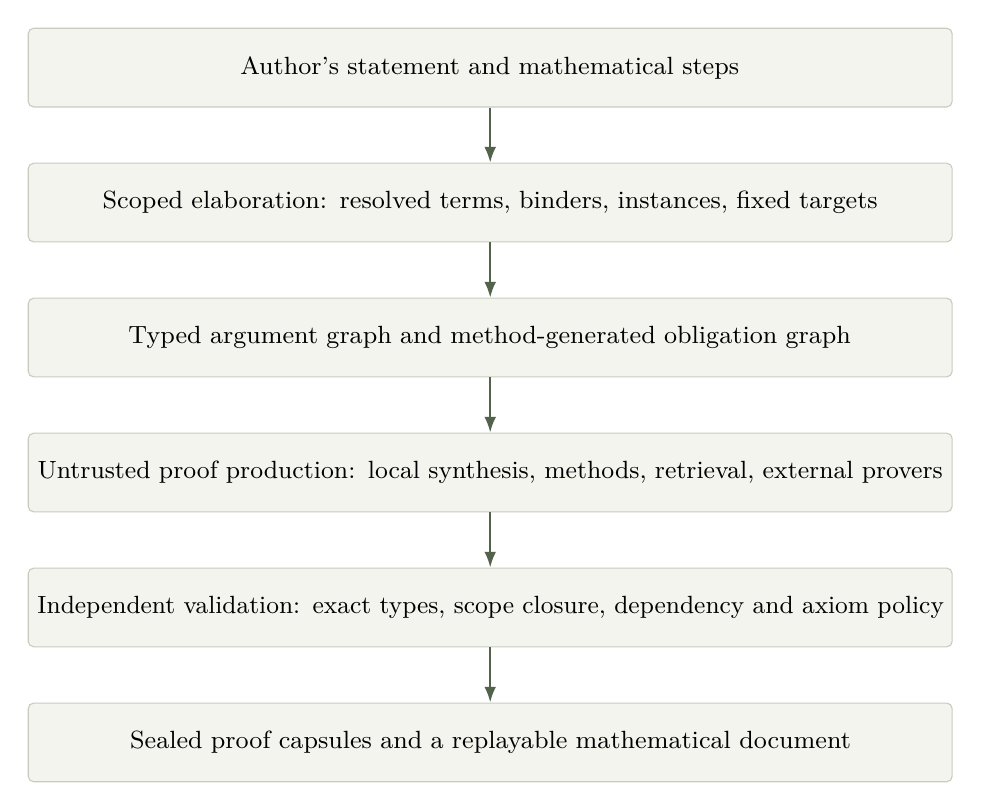
\begin{tikzpicture}[
 node distance=7mm,
 box/.style={draw=rulegray,rounded corners=2pt,fill=light,text width=11.5cm,minimum height=10mm,align=center,font=\small},
 arr/.style={-{Latex[length=2mm]},draw=accent,thick}]
\node[box] (source) {Author's statement and mathematical steps};
\node[box,below=of source] (meaning) {Scoped elaboration: resolved terms, binders, instances, fixed targets};
\node[box,below=of meaning] (ir) {Typed argument graph and method-generated obligation graph};
\node[box,below=of ir] (search) {Untrusted proof production: local synthesis, methods, retrieval, external provers};
\node[box,below=of search] (check) {Independent validation: exact types, scope closure, dependency and axiom policy};
\node[box,below=of check] (capsule) {Sealed proof capsules and a replayable mathematical document};
\foreach \a/\b in {source/meaning,meaning/ir,ir/search,search/check,check/capsule}
  \draw[arr] (\a) -- (\b);
\end{tikzpicture}
\caption{Proposed architecture. A search result cannot alter a previously fixed target or become a new assumption. Feedback from failed checking goes to reconstruction, not to silent reinterpretation.}\label{fig:pipeline}
\end{figure}

\subsection{Goal requests should be self-contained}
A synthesis request should identify an immutable task rather than depend on the worker's accidental current session:
\Needspace{166pt}
\begin{code}
SynthesisRequest {
  requestId          : RequestId
  targetIdentity     : GoalIdentity
  closedTelescope    : SerializedTelescope
  target             : SerializedExpr
  permittedProviders : ProviderInventory
  methodProfile      : VersionedProfileId
  environment        : EnvironmentFingerprint
  axiomPolicy        : PolicyId
  workBudget         : WorkBudget
  expectedOutput     : Proof | WitnessWithSpecification
}
\end{code}
A response contains either a candidate associated with this exact request or a qualified failure. Provider identities include the instantiated declaration, universe arguments, and local-context bindings. It is not enough to return a theorem name plus a list of loosely correlated strings.

Within a Lean worker, the natural representation is elaborated expressions. Across a process boundary, local free-variable identifiers must be replaced by explicit telescope positions or another validated binding representation. Decoding reconstructs the context, checks every binder type, and rechecks the candidate. Raw memory references, pretty-printer output, and session-local metavariable identifiers cannot serve as portable authority.

\subsection{A disciplined search schedule}
A practical default schedule is: replay an exact cached certificate; try cheap structural closure; invoke the selected syntax-directed domain method; solve its side conditions with small local procedures; then attempt bounded provider synthesis. Broader retrieval or learned strategic search is invoked explicitly or under a clearly named exploratory profile.

The order is a policy, not a soundness assumption. Any returned candidate goes through the same checking boundary. Nevertheless, the order matters for predictability and cost. An expensive domain-independent search should not run before a direct chain-rule reconstruction on an elementary derivative expression.

Within a domain method, search can be specialized. Arithmetic facts go to arithmetic procedures; conjunction plumbing goes to constructor synthesis; an expression identity goes to an equality-producing normalizer. This is not merely an optimization. It allows the system to report which mathematical subtask failed and what additional hint would reduce the search space.

A budget needs more than wall-clock time. Candidate count, expansion count, simplification fuel, provider count, recursion depth, memory, and verifier cost can matter. Logical status must never depend on interpreting a resource limit as evidence of impossibility. Cancellation may discard speculative work, but cannot invalidate an already checked, correctly scoped proof capsule.

\subsection{Isolation and transaction boundaries}
Each speculative branch owns its elaboration state. Failure restores that state before another branch is tried. However, restoring a metavariable context is not sufficient when a tactic can change global declarations or perform external I/O. Search workers should therefore operate against immutable base environments, and any proposed new declaration should be returned as data for separate validation.

The final verifier should not rerun arbitrary unreviewed tactic code merely to discover what theorem was supposedly proved. It should consume a validated, closed proof representation, or a controlled proof-reconstruction language whose operations cannot mutate the target environment arbitrarily. Generated support lemmas are acceptable only when their types and proofs are independently checked and their dependency graph is acyclic or uses a checked recursive definition.

The project's configured worker executables and imported libraries remain explicit operational dependencies. The language should not discover a new executable or authorize network access because a proof step contains a suggestive phrase. External tool permissions are a session or project policy, not part of the mathematical syntax.

\subsection{Candidate ranking should preserve explanation choices}
Leant already distinguishes ranking policies, and its verification scheduler preserves accepted representatives of candidate groups.\cite{leant-readme,leant-verification} For \ms, a useful score can consider proof-term size, dependency breadth, reconstruction cost, and correspondence to the selected method. But ranking should not silently replace a declared intermediate assertion by an unrelated direct proof of the final theorem.

For instance, if the author wrote the positive-square-root argument, a candidate using the recorded square identity and branch fact is a better fit than one invoking a previously proved uniqueness theorem that bypasses those steps. The bypass can be offered as an alternative proof, but it changes the explanatory structure.

This is a constrained synthesis problem: the source graph fixes certain intermediate interfaces, and the synthesizer fills the remaining edges. One can call the graph a \emph{proof sketch}, provided that all its holes have exact types and every chosen assertion remains independently checkable.

\section{Trust, assumptions, and statement fidelity}\label{sec:trust}

\subsection{Three boundaries, not one slogan}
``The kernel checks it'' is a necessary design principle, but it does not answer every trust question. The architecture should distinguish three boundaries.

The \textbf{logical boundary} asks whether the supplied term proves the fixed proposition relative to the approved foundation. The \textbf{meaning boundary} asks whether that proposition and its definitions express the intended mathematics. The \textbf{execution boundary} asks whether running the proof-producing software can modify the environment, interfere with validation, or perform unwanted operations.

Lean's current validation guidance explicitly distinguishes validity of a proof from meaning of its statement and describes escalating rechecking options, including a trusted challenge statement and independently checked exported evidence.\cite{lean-validation} \ms\ should build this distinction into its architecture rather than add it only as a late audit feature.

The logical trusted base includes the chosen checker and its accepted foundational rules and axioms. The meaning boundary additionally involves the declared definitions, elaboration configuration, and the user's acceptance of the resolved statement. Operational protections concern worker isolation and validation infrastructure. A small logical kernel does not make all three boundaries identical.

\subsection{Axiom policy should be an allowlist}
The policy should compute the transitive axiom dependencies of the final declaration, including dependencies of used theorems and definitions, and compare them with an explicit allowlist. Different projects can choose different foundations; a real-analysis project may permit standard classical mathematical axioms, while a constructive development may impose a narrower policy.\cite{lean-axioms}

The policy must reject unfinished proofs and unapproved generated axioms. Checking only for one historical name is insufficient. Current Lean documentation notes that, since Lean 4.29, native-computation assertions can introduce computation-specific axioms rather than the older single \ty{Lean.trustCompiler} dependency.\cite{lean-validation} This matters for a project pinned to 4.32: a validator that merely bans the older name would not express a kernel-only evidence policy.

The proposed default is therefore structural: only the declared foundational axioms are accepted. A fast external computation is welcome when it produces evidence that the configured checker can validate without enlarging that policy. A project may deliberately opt into additional trusted computation, but the resulting status and assumptions must be different and visible.

User hypotheses should ordinarily appear as theorem parameters, not as fresh global axioms. This makes the difference between ``we proved $P$ under assumptions $H$'' and ``we silently enlarged the foundation'' explicit in the declaration itself.

\subsection{Definitions are part of the statement}
A theorem about \ty{Continuous} is only as meaningful as the resolved definition of that predicate. A target involving a custom division operator or a weakened notion of convergence may be perfectly provable and still differ from the intended mathematics.

For important theorems, \ms\ should support a trusted target file or declaration fingerprint fixed independently of the proof-producing session. The final result is compared against that target after elaboration in the intended environment. Where a surface translation claims to preserve an existing Lean theorem, the comparison should be definitional equality of the elaborated statements when possible, or an explicitly checked equivalence when the presentation changes the formulation.

An equivalence proof is not permission to rename an arbitrary theorem as the user's target. Its assumptions, quantifier structure, and dependency policy must be checked, and the relationship should be visible in the artifact. Exact preservation is the simplest default for the ProveIt migration examples.

\subsection{Explanatory fidelity is not ordinary logical soundness}
Suppose a source says ``by the chain rule,'' but the checker accepts a proof using an unrelated black-box theorem. The result can be logically valid while the explanation is misleading. No general-purpose proof checker automatically decides whether a human explanation is a faithful account of all semantic dependencies.

The initial design should offer a modest, enforceable guarantee: the named method produced a checked reconstruction plan with specified intermediate claims, and the displayed explanation is generated from that plan. Free prose remains commentary. A stronger claim that the generated prose captures a human's actual reasoning process would not be justified.

The author can insist on a particular mathematical path by retaining its intermediate assertions. The system can lint unused assertions, unexpected dependencies, or a method that was bypassed during fallback. These are useful diagnostics, but not a decision procedure for the best or most explanatory proof.

\section{Freeze the proof, not the search}\label{sec:freeze}

\subsection{Discovery mode and sealed mode}
A proof has two operational states. In \emph{discovery mode}, methods may search, request suggestions, try alternatives, and leave unresolved obligations. In \emph{sealed mode}, every assertion has a fixed interpretation and a checked proof capsule. Rechecking sealed mode does not invoke synthesis.

This separation answers a common concern about concise proof languages: if a short line depends on a sophisticated search engine, will the proof still build after a heuristic change? The answer should be that search is used to create or repair the proof, not to rediscover it during every verification run.

Sealing does not promise that proof checking is free. A large proof term or expensive reduction can still be costly. It promises that the accepted result is independent of the current suggestion model and search order, subject to the same pinned definitions, checker semantics, and sufficient checking resources.

\subsection{Contents of a proof capsule}
A capsule should include the closed target, the closed proof or a checkable reconstruction certificate, universe parameters, transitive dependency identities, the axiom inventory, and a source-to-evidence map. The enclosing artifact records the toolchain and policy. A source lock can additionally retain method selections and normalized expression identities used to detect changes.

An illustrative manifest is:
\Needspace{142pt}
\begin{code}
proof_capsule:
  schema: mathstep-capsule-1
  target: <closed typed expression>
  telescope: <ordered source inputs and local definitions>
  proof: <validated proof representation>
  dependencies: <exact declaration identities>
  axioms: <computed transitive inventory>
  method: <versioned method and resolved theorem bindings>
  source_map: <step IDs to proof and obligation nodes>
  toolchain: <exact checker and library revisions>
\end{code}
This is not a suggestion to trust a JSON field named \ty{axioms}. The verifier recomputes or validates the dependency information from the actual evidence. Metadata can accelerate checking and improve explanations; it cannot substitute for the evidence it describes.

A compiled \ty{.olean} file is a useful toolchain-specific artifact, not by itself a universal, implementation-independent certificate format. A mature implementation can offer both native replay artifacts and a validated export format. The article does not prescribe a new binary proof format before a prototype has measured the relevant term sizes and checker costs.

\subsection{Cache keys and invalidation}
A safe positive-certificate key must bind at least the target expression, local telescope, relevant declarations and their meanings, universe assignments, and logical policy. A discovery cache additionally needs the available provider inventory, method versions, elaboration options, and resource policy, because those influence what was searched.

Alpha-normalized structural serialization is a reasonable basis for hashing. It need not compute a universal canonical normal form modulo definitional equality. Different but definitionally equal expressions can simply miss the cache and be checked again; conservative misses are preferable to unsafe hits.

Adding an irrelevant theorem to the environment need not invalidate a sealed proof whose exact dependencies are unchanged. Changing a used definition, type-class instance, recursor, or theorem statement does. A local hypothesis can sometimes be renamed or the context weakened while preserving a certificate, but such reuse requires an explicit scope mapping and rechecking, not a string substitution in the stored proof.

Negative search caches need stricter keys. ``No candidate within this budget'' refers to a particular inventory, method policy, and bounded search. Reusing it after new relevant facts are introduced would be misleading. Even under an exact key it remains a search receipt, not a mathematical refutation.

\subsection{Repair is an explicit operation}
When a dependency changes, sealed mode reports which nodes no longer match. Repair mode may rerun synthesis for the invalidated region while preserving unaffected assertions and certificates. Any changed intermediate statement is presented as a mathematical edit, not hidden in a regenerated lock file.

A useful semantic diff separates changes to the theorem statement, definitions, explicit assumptions, chosen intermediate assertions, axiom inventory, method bindings, and low-level proof evidence. A change only in an arithmetic normalization certificate deserves different attention from a changed branch hypothesis.

This gives concise proofs a plausible maintenance story. The durable document contains mathematical interfaces, and repair regenerates implementations of those interfaces. The approach resembles a compiler preserving a typed intermediate contract, not a prose document repeatedly reinterpreted from scratch.

\section{Interaction: the proof as an inspectable document}\label{sec:interaction}

\subsection{Three synchronized views}
The editor should offer a mathematical view, an obligation view, and a fully elaborated view. These are presentations of one typed document, not independently maintained files.

The mathematical view shows the author's assertions, calculations, and named methods. The obligation view shows generated premises and their status. The elaborated view shows exact Lean targets, terms, dependencies, and assumptions. A reader can move from ``differentiate on $s$'' to the neighborhood equality and then to the precise theorem applications without losing the source location.

A static PDF export can preserve the first view and selectively include the second for important steps. An accompanying machine-checkable artifact carries the third. The PDF's typography should not itself be treated as the proof certificate; the association between displayed claims and typed nodes must be explicit in the generated source map.

\subsection{Suggestions should explain their scope}
A suggestion is more useful when it states what it proposes to solve. Compare ``try a stronger tactic'' with:
\Needspace{58pt}
\begin{code}
The current induction hypothesis is specialized to x.
Suggested change: generalize x before induction on n.
This supplies equality on s, from which locality can prove equality near x.
\end{code}
The second suggestion changes the proof structure, so it should be shown as a source edit with its resulting motive. Another suggestion might only discharge a denominator obligation and can be accepted as a local reconstruction without changing the mathematical text.

The interface should distinguish a proved suggestion, a partially reconstructed plan, a proposed statement not yet proved, and a rejected candidate. A generated explanation should not describe a candidate as established before all its obligations are checked.

\subsection{Do not punish local experimentation}
An author should be able to introduce a tentative lemma, inspect its implications, and later replace it. Such exploratory assumptions must have a visibly different status from proved assertions and may not flow into a sealed theorem unnoticed.

The simplest implementation is to treat an unproved lemma as an open obligation node rather than adding a new axiom to the accepted environment. Dependent results remain provisional. Sealing fails with the unresolved dependency path, even if the last visible proof block has no holes.

This supports the natural workflow of mathematics without weakening the final artifact. The system need not forbid sketches; it needs to distinguish sketches from completed proofs in its data model.

\subsection{Explain the missing mathematics, not only the API mismatch}
A good diagnostic reports the failed mathematical precondition and then offers lower-level detail. Examples include ``the denominator may be zero,'' ``the equality is only pointwise,'' ``the chosen witness depends on a variable outside its scope,'' and ``this substitution changes the index of a dependent type.''

The raw elaborator message remains available for experts. But the domain method owns enough information to attach a useful explanation to an error before the user has to inspect an internal metavariable name or a long chain of instance arguments.

\section{Prior art and the actual design contribution}\label{sec:prior}

\subsection{Declarative proof languages are an established idea}
Isar is explicitly designed for structured, intelligible, semi-automated reasoning. Its existence is a reminder that readable proof documents and rigorous checking are not opposing goals.\cite{isar} Mizar likewise provides an established mathematical vernacular, while Naproche explores controlled mathematical language and implicit-information processing in ordinary-looking mathematical texts.\cite{mizar,naproche}

\ms\ is not presented as the first declarative proof language or the first attempt at controlled mathematical prose. Its proposed contribution is a particular integration: typed mathematical-step contracts, scoped obligation tracking, a synthesis interface with explicit evidence strengths, and sealed reconstruction artifacts within the Lean ecosystem.

\subsection{Lean-specific work is especially relevant}
Aesop provides configurable rule-based proof search with normalization and distinctions between safe and backtracking search rules. It is a natural candidate backend for suitable local tasks, not a competitor that must be replaced.\cite{aesop} Verbose Lean explores controlled natural-language presentations in Lean and is relevant to the surface-language and teaching aspects of the design.\cite{verbose}

Lean blueprints connect mathematical exposition and formal developments through structured documentation.\cite{blueprint} \ms\ would differ by making the accepted mathematical steps themselves part of an elaborated, checkable source graph, rather than only organizing an informal document around formal declarations. Blueprint-style exposition remains valuable for motivation and large-scale proof planning.

Leant supplies the most directly relevant engineering experience for the proposal: type-directed candidate construction, tactic suggestions, fragment boundaries, exact-goal validation, provenance, and conservative handling of negative results. The proposed language changes the granularity at which those mechanisms are offered to the author.\cite{leant-readme,leant-internals}

\subsection{External automation needs reconstruction, not a new foundation}
The lean-smt approach and work on SMT proof reconstruction in Isabelle illustrate a broader pattern: external reasoning can be powerful while its result is reconstructed inside the assistant.\cite{lean-smt,smt-reconstruction} \ms\ adopts that pattern at the level of mathematical methods and intermediate assertions.

The main unresolved challenge is therefore not inventing a new notion of proof validity. It is designing a good contract between an author, a mathematical library, a family of proof-producing tools, and a stable checker. A claim of novelty would require a wider literature study than this source-grounded design review; the implementation should be judged first on whether that contract improves actual mathematical work.

\section{Implementation plan: a Lean-hosted frontend first}\label{sec:implementation}

\subsection{Recommended boundary of the first implementation}
The initial implementation should be a Lean package, not a new kernel or an independent replacement for Lean's type system. It should retain ordinary Lean declarations and introduce a \ty{mathstep} proof block. An escape hatch should allow a local proof to be supplied in ordinary Lean, with exactly the same certificate and assumption checks as a generated proof.

Start with \ty{have}, \ty{calc}, and \ty{suffices}, plus ordinary introduction and case syntax delegated to Lean. These are enough to test the central hypothesis that stable mathematical assertions plus local reconstruction improve authoring. Do not begin by implementing unrestricted natural language, autonomous theorem discovery, a new module system, and a new proof serialization format at once.

A minimal module layout could be:
\Needspace{154pt}
\begin{code}
MathStep.Syntax           -- parser and source identities
MathStep.Elab             -- scoped target elaboration
MathStep.Graph            -- argument and obligation nodes
MathStep.Method           -- method interface and registry
MathStep.Methods.Algebra  -- equality-producing normalization
MathStep.Methods.Calculus -- derivative and locality plans
MathStep.Methods.Binders  -- finite-sum congruence traversal
MathStep.Synth            -- provider requests and outcomes
MathStep.Verify           -- final checks and policy acceptance
MathStep.Capsule          -- sealed artifacts and invalidation
MathStep.Info             -- explanations and source maps
\end{code}
These are proposed module names, not files claimed to exist in either inspected repository.

\subsection{Milestones defined by evidence, not dates}
\textbf{Milestone 1: typed assertions and replay.} Implement the small core with exact target preservation, ordinary Lean reconstruction, obligation states, and a simple sealed-artifact path. Demonstrate that a proof can be rechecked after disabling the search service. Establish rejection tests for unresolved holes, escaped variables, and unapproved axioms before adding sophisticated automation.

\textbf{Milestone 2: one elementary domain pack.} Implement real algebra with explicit nonzero and square-root guards, then syntax-directed differentiation of the root example. Keep both the concise step and the expanded proof trace. Compare against an expert Lean proof using the same helper lemmas.

\textbf{Milestone 3: a Leant adapter.} Connect local completion requests to Leant's existing synthesis boundary. Preserve opaque dependent-expression identity and exact provider bindings. Distinguish candidate acceptance stages and negative-result strengths. Keep a direct Lean backend available so that the language does not depend on successful translation into a single fragment.

\textbf{Milestone 4: scoped mathematical operations.} Implement locality promotion, derivative congruence, and finite-sum substitution with binder-aware side conditions. Use the autonomous-ODE and dyadic bridge examples as integration tests, preserving the original theorem statements exactly.

\textbf{Milestone 5: structured induction completion.} Add explicit motive presentation and ``rebuild remaining constructors'' for the natural-deduction example. Freeze case coverage, validate contextual indices, and test invalidation when the inductive definition changes.

\textbf{Milestone 6: evaluation and interface refinement.} Measure authoring, comprehension, repair, search, and replay against controlled baselines. Only after those results should the project expand the prose grammar or add learned strategic suggestions as a default workflow.

\subsection{Why a native worker is attractive, but not mandatory initially}
A Lean-native worker can retain elaborated expressions, local contexts, and inference state without repeatedly converting through text. That makes the proposed identity and scope discipline easier to implement. It also allows method reconstruction to reuse the existing mathematical environment directly.

This does not imply that the entire Djex search engine must be rewritten before \ms\ is useful. A narrow bridge can send a restricted structural problem to the existing engine and reconstruct the result in Lean. The bridge should advertise its supported fragment and preserve all source identities that the final check needs. Rewriting the engine is an independent engineering decision whose cost should be justified by measurements rather than assumed necessary for a better surface language.

\subsection{Support lemmas should be ordinary library assets}
Whenever a method repeatedly needs the same mathematical bridge, such as equality on an open set implying equality near a point, that bridge should be an ordinary named theorem where feasible. The method then concerns recognition, instantiation, obligation management, and presentation.

This division prevents method implementations from accumulating large amounts of hidden mathematics. It also benefits ordinary Lean users, provides a fair comparison baseline, and allows a domain pack to be audited separately from the search policy. A method whose value disappears once its helper lemmas are exposed may still be a useful interface, but its claimed advantage should be described accordingly.

\section{Evaluation: how to tell whether the language is better}\label{sec:evaluation}

\subsection{A controlled baseline matrix}
The central empirical question is not whether the proposed syntax is shorter than a particular existing script. It is whether it reduces effort while preserving correctness, clarity, and maintainability. The evaluation should include:
\begin{center}
\begin{tabularx}{\linewidth}{@{}L{.23\linewidth}YY@{}}
\toprule
Condition & Source language & Available proof machinery\\
\midrule
Original source & Pinned ProveIt Lean & Original library and proof.\\[3pt]
Expert refactoring & Ordinary Lean & Same mathematical content, idiomatic refactoring.\\[3pt]
Shared automation & Ordinary Lean & All helper lemmas and methods also available to \ms.\\[3pt]
Mathematical steps & \ms & The same machinery, plus step syntax, ledger, and sealing.\\
\bottomrule
\end{tabularx}
\end{center}
Leant and learned strategic search should be separately enabled or disabled in paired experiments. Otherwise an improvement due to a stronger prover could be mistaken for an improvement due to the language.

The original and translated statements should be compared at the elaborated level. A theorem proved under stronger hypotheses, a changed branch convention, or a weakened definition is not a successful compression of the original theorem. A change in permitted foundational axioms must also be reported.

\subsection{Metrics that capture the real tradeoff}
Measure author-written tokens, number of edit-and-check iterations, time spent locating or adapting lemmas, number of manually supplied side conditions, and repair effort after controlled library changes. For readers, measure whether they can identify the induction motive, domain conditions, branch choice, and main dependency without expanding every generated detail.

For the implementation, measure median and tail discovery time, time to the first checked candidate, peak memory, number of attempted candidates, proof size, replay time, and cache invalidation locality. These are different quantities. A method that is expensive once but cheap to replay may be valuable; a tiny source step that generates an enormous certificate may be a poor default.

The supporting library must be included in the accounting. Report both per-proof source size and the amortized cost of domain packs over a corpus. A concise proof should not be credited with eliminating work that has merely been moved into a new handwritten theorem specific to that proof.

The article reports no measured compression percentage or speedup. The examples are concrete design targets and mathematical reconstructions, not a completed benchmark.

\subsection{A rejection corpus is as important as a success corpus}
The following cases should be regression tests from the beginning. Some are false mathematical transformations; others test scope or evidence policy. Rejection does not always mean the intended theorem is false: it can mean that a requested method lacks sufficient evidence.
\begin{longtable}{@{}L{.30\linewidth}L{.31\linewidth}L{.33\linewidth}@{}}
\toprule
Mutation or attempted step & Why it is problematic & Required behavior\\
\midrule
\endhead
Drop the nonnegative-radicand condition in the root equation. & $q=-1$ is a counterexample to the unrestricted equation. & Do not apply the square-root square identity without evidence.\\[4pt]
Drop the branch condition in root uniqueness. & At $q=0$, the second root is $-1/4$. & Retain a sign obligation; do not infer a branch from a squared identity.\\[4pt]
Differentiate equality only at a point. & $t$ and $0$ agree at $0$ but their derivatives differ. & Require local equality or a separate suitable theorem.\\[4pt]
Normalize natural subtraction without $k\leq N$. & $N=1,k=2$ refutes the intended cast identity. & Generate and discharge the cast guard.\\[4pt]
Move an $\varepsilon$-dependent choice outside its scope. & The quantifier order changes. & Reject escaping dependencies or show an explicit reformulation.\\[4pt]
Treat failed fragment search as a proof of $\neg P$. & Search failure and logical negation are different statements. & Return a qualified search status only.\\[4pt]
Reuse a certificate after changing a used definition or instance. & The apparent target can acquire a different meaning. & Invalidate and recheck against the new target.\\[4pt]
Add a constructor to an inductive relation. & Previously exhaustive case coverage is no longer exhaustive. & Invalidate constructor-coverage evidence.\\[4pt]
Accept a theorem through an unproved dependency. & A locally finished proof can depend on a hole or new axiom. & Audit the transitive dependency closure.\\[4pt]
Return the wrong projection of $A\to A\to A$. & The type permits several computations. & Check the stated behavioral specification, not just the type.\\
\bottomrule
\end{longtable}
A useful additional test mutates the displayed notation while leaving a superficially similar theorem in place. This tests the meaning boundary rather than the proof search. Another replaces a callback's accepted candidate with a differently rendered candidate to test that evidence is attached to the exact object, not copied across a convenient string match.

\subsection{Generalization beyond the motivating examples}
A prototype can easily overfit a handful of attractive demonstrations. The next evaluation corpus should contain unfamiliar examples in algebra, finite combinatorics, elementary topology, and analysis. Domain packs should be developed on one subset and tested on another.

The strongest evidence of a language improvement would be repeated use of the same small method contracts across unrelated theorems, with users supplying fewer low-level adapters while still understanding why the methods apply. A system that only shortens examples after a bespoke theorem has been written for each one has demonstrated abbreviation, not general improvement in proof authoring.

\section{Limits and research questions}\label{sec:limits}

\subsection{The library remains the main source of mathematical knowledge}
A concise phrase such as ``by compactness'' depends on a substantial body of definitions and theorems. The language cannot eliminate that work. It can make the relevant theorem easier to select, instantiate, inspect, and reuse. A high-quality domain pack therefore requires mathematical library engineering as well as parser and search engineering.

One open design question is how to distribute effort between explicit method schemas and learned retrieval. Schemas give predictable obligations and explanations; learned retrieval can cover a much larger vocabulary. The proposed architecture permits both, but requires the learned path to resolve to explicit checked claims before acceptance.

\subsection{Concision and locality can conflict}
A powerful global prover may close a goal that a carefully restricted local method cannot. Allowing it everywhere can reduce author input while making proofs less predictable and less explanatory. Conversely, a very strict local policy may force users to spell out obvious connections.

This suggests configurable profiles rather than a single universal setting. A lecture-style proof may retain more intermediate steps. A computational certificate may prioritize replay efficiency. A research notebook may permit broad exploration while a publication artifact requires every method and dependency to be sealed. The formal target and acceptance policy remain explicit in every profile.

\subsection{There is no general automatic test for a good explanation}
Logical soundness is sharply defined; explanatory adequacy is not. The argument graph provides a useful intermediate object, but deciding which steps a reader needs depends on prior knowledge. The editor should therefore support adjustable detail and user-controlled mathematical anchors rather than assume that the smallest proof term is the best explanation.

A promising research direction is explanation-preserving proof compression: simplify evidence while preserving a selected graph of assertions and method contracts. This is more constrained than searching for any proof of the final proposition, and more meaningful than merely shortening a tactic script. Its quality still needs human evaluation.

\subsection{Certifying the frontend itself is a later, separate project}
The small-core soundness argument suggests a route to formalizing parts of the frontend: a typed core syntax, its elaboration into a host calculus, and proofs that scope-preserving transformations retain meaning. But a full Lean elaborator, extensible notation environment, and interactive editor are much larger targets.

The practical first guarantee comes from checking output against a fixed statement, not from proving the entire implementation correct in advance. Formal verification of selected frontend transformations can strengthen that guarantee over time. It should not be confused with verification of the mathematical theorem or with evidence that the interface is easier to use.

\section{Recommendation}\label{sec:conclusion}
The most promising design is not ``Lean with fewer keywords'' and not ``English that a model says is correct.'' It is a declarative layer whose mathematical steps have exact types, scoped preconditions, and checkable reconstructions.

For ProveIt, the first useful methods are already visible in the inspected code: guarded algebra and differentiation of an explicit branch; promotion from an identity on an open set to a local identity; substitution under a finite-sum binder with its index facts; and reconstruction of routine induction cases. Each has a small mathematical contract and a concrete existing Lean proof that can serve as a reference target.

For Leant, the opportunity is to make structural synthesis and tactic suggestion services of this step language. Keep the exact-goal validation discipline, the distinction between positive reconstruction and negative search evidence, and the careful provenance boundaries. Strengthen the frontend around typed assertion graphs, explicit witness specifications, independent statement identity, and sealed proof artifacts.

The initial implementation should therefore be modest in syntax and ambitious in its contracts: a Lean-hosted frontend, a few reusable domain methods, a scoped obligation ledger, a precise Leant bridge, and search-free replay. Evaluate it against ordinary Lean supplied with the same mathematical tools.

\begin{quote}
\textbf{Write the mathematical choices. Reconstruct the bookkeeping. Check the exact claim. Preserve the reconstruction.}
\end{quote}
That is a concrete route toward proofs that look more like mathematics without requiring the reader or the machine to take an omitted argument on trust.

\appendix
\clearpage
\section{A deliberately small core grammar}\label{app:grammar}
The following EBNF describes a proposed core, not all the richer domain notation shown earlier. \ty{Term}, \ty{Type}, and \ty{Prop} are delegated to the host expression elaborator. Indentation or explicit delimiters can provide blocks; the semantic scope is identical.
\Needspace{262pt}
\begin{code}
Proof       ::= "proof" Block "end"
Block       ::= Step* Close
Step        ::= "take" Binder
              | "assume" Name ":" Prop
              | "let" Name [":" Type] ":=" Term
              | "have" Name ":" Prop Justification
              | "choose" Binder "with" Name ":" Prop "from" Term
Close       ::= "show" Prop Justification
              | "show" "thesis" Justification
              | "calc" Calculation
              | "suffices" Name ":" Prop "then" Block "prove" Block
              | "cases" Term "with" Branch+
              | "induct" Term ["generalizing" Name*] "with" Branch+
Justification ::= "by" Method [Premises]
                | Premises "by" Method
                | "by" "lean" HostProof
                | "by" Proof
Premises    ::= "from" TermList
              | "using" ["only"] TermList ["with" Profile]
Branch      ::= "|" Pattern "=>" Block
\end{code}
A \ty{suffices} construct supplies a continuation from the intermediate claim to the outer goal and a proof of that claim. A \ty{choose} extends only the continuation's local scope. A \ty{cases} or \ty{induct} discharges the selected current goal through its checked branches; the surrounding block cannot reuse branch-local assumptions as outer facts. Surface desugaring must make these scope boundaries unambiguous.

Method calls and domain notation may extend the grammar, but they may not extend the set of accepted logical rules. A new phrase lowers to a checked method plan or ordinary core constructs. An unknown phrase is a syntax or method-resolution error, not an invitation to infer an axiom from prose.

\clearpage
\section{The completion algorithm as an interface contract}\label{app:algorithm}
The following pseudocode specifies responsibilities, not concrete Lean API names.
\Needspace{418pt}
\begin{code}
complete(step, immutableEnvironment, policy):
  target := elaborateDeclaredTarget(step, immutableEnvironment)
  require target has a well-formed scoped telescope
  require target interpretation matches the accepted source identity

  cached := lookupExactCapsule(target, immutableEnvironment, policy)
  if cached exists and independentCheck(cached, target, policy):
    return PolicyAccepted(cached)

  if policy.mode == Sealed:
    return NeedsRepair(step.id)

  for plan in boundedPlans(step, target, policy):
    branch := isolatedStateFor(target, immutableEnvironment)
    obligations, reconstruction := elaboratePlan(plan, branch)
    require every obligation has an owner and a well-formed scope
    require obligation dependencies are acyclic after scope closure

    proofs := completeObligations(obligations, policy)
    if any obligation remains unresolved:
      retainDiagnostic(plan, unresolvedObligations)
      continue

    candidate := assemble(reconstruction, proofs)
    require candidate has no unresolved expression or universe metavariables
    closed := closeOverDeclaredTelescope(candidate)

    checked := independentCheck(closed, target, policy)
    if checked succeeds:
      capsule := sealExactEvidence(checked, step.sourceMap)
      return PolicyAccepted(capsule)

  return NoReconstructionWithinPolicy(retainedDiagnostics)
\end{code}
The independent check validates the candidate's type, declared inputs, relevant dependencies, and axiom policy. The algorithm never responds to a failed proof by weakening the target. Recursive calls used to discharge method obligations are bounded search, not proof-level recursion; their termination policy is operational. Any mathematical induction appears explicitly in the candidate's checked recursor applications.

\clearpage
\section{Exact source map for the case studies}\label{app:sourcemap}
\begingroup\raggedright
All ProveIt entries below refer to commit \texttt{\pv}. All Leant entries refer to \texttt{\lv}.

\textbf{Algebraic branch.} The relevant ProveIt declarations are \ty{dyadicRootFun}, \ty{dyadicRootFun\_solves}, \ty{eq\_dyadicRootFun\_of\_solves}, and \ty{hasDerivAt\_dyadicRootFun\_zero} in \ty{AlgebraicInverseGermAnalytic.lean}. The article's positive-square-root uniqueness argument is an alternative proof of the same implication, not a description of the source's factorization script.\cite{proveit-root}

\textbf{Autonomous derivative family.} The main reference is \ty{AutonomousODE.iteratedDeriv\_eq\_comp} in \ty{AutonomousIteratedDeriv.lean}. The article preserves its range-restricted derivative hypotheses. The source also contains a wrapper under globally differentiable-family assumptions; that stronger wrapper is not used to replace the more general main statement.\cite{proveit-ode}

\textbf{Dyadic substitution.} The reference declarations are \ty{rvachevUp\_dyadic\_eq\_qBinomial} and \ty{foldedCoefficient\_two\_pow\_eq\_qBinomial} in \ty{AliasQBinomialBridge.lean}. The symbols $u,F,Q,A$ in the exposition are reader-facing aliases, and the suppressed casts are described in Section~\ref{sec:dyadic}.\cite{proveit-alias}

\textbf{Natural deduction.} The reference is \ty{LeanProofs.NaturalDeduction.Derives.mapAxioms} in \ty{Logic/Propositional/NaturalDeduction/Lean/NaturalDeduction/Calculus.lean}. The proposed generic completion must preserve the recursor's contextual indices in all eleven branches.\cite{proveit-nd}

\textbf{Leant boundaries.} The reviewed files are the pinned \ty{README.md}, \ty{docs/synth-internals.md}, \ty{src/Leant/Synth/Verification.hs}, and the initial representation and translation documentation in \ty{src/Leant/Synth/Fragment.hs}. The present article does not claim to have audited the full backend or independently reproduced the repositories' acceptance-test reports.\cite{leant-readme,leant-internals,leant-verification,leant-fragment}

\par\endgroup
\newpage
\begin{thebibliography}{99}
\addcontentsline{toc}{section}{References}
\small\raggedright

\bibitem{proveit-toolchain}
Vladimir Reshetnikov and contributors. \emph{ProveIt: lean-toolchain}. Commit \texttt{\pv}.
\url{https://github.com/VladimirReshetnikov/ProveIt/blob/24ce8bd743eaab64a91ce90725ea00f498d319d2/lean-toolchain}.

\bibitem{proveit-root}
Vladimir Reshetnikov and contributors. \emph{ProveIt: AlgebraicInverseGermAnalytic.lean}. Commit \texttt{\pv}.
\url{https://github.com/VladimirReshetnikov/ProveIt/blob/24ce8bd743eaab64a91ce90725ea00f498d319d2/Analysis/FabiusFunction/Lean/FabiusFunction/AlgebraicInverseGermAnalytic.lean}.

\bibitem{proveit-ode}
Vladimir Reshetnikov and contributors. \emph{ProveIt: AutonomousIteratedDeriv.lean}. Commit \texttt{\pv}.
\url{https://github.com/VladimirReshetnikov/ProveIt/blob/24ce8bd743eaab64a91ce90725ea00f498d319d2/Analysis/FabiusFunction/Lean/FabiusFunction/AutonomousIteratedDeriv.lean}.

\bibitem{proveit-alias}
Vladimir Reshetnikov and contributors. \emph{ProveIt: AliasQBinomialBridge.lean}. Commit \texttt{\pv}.
\url{https://github.com/VladimirReshetnikov/ProveIt/blob/24ce8bd743eaab64a91ce90725ea00f498d319d2/Analysis/FabiusFunction/Lean/FabiusFunction/AliasQBinomialBridge.lean}.

\bibitem{proveit-nd}
Vladimir Reshetnikov and contributors. \emph{ProveIt: NaturalDeduction/Calculus.lean}. Commit \texttt{\pv}.
\url{https://github.com/VladimirReshetnikov/ProveIt/blob/24ce8bd743eaab64a91ce90725ea00f498d319d2/Logic/Propositional/NaturalDeduction/Lean/NaturalDeduction/Calculus.lean}.

\bibitem{leant-readme}
Vladimir Reshetnikov and contributors. \emph{Leant: README}. Commit \texttt{\lv}. In particular, interactive proving, the synthesis fragment, and verification and negative-result qualifications.
\url{https://github.com/VladimirReshetnikov/Leant/blob/c36adf114035fb2fba6c276b63944cc613b31668/README.md}.

\bibitem{leant-internals}
Vladimir Reshetnikov and contributors. \emph{Leant: :synth internals}. Commit \texttt{\lv}.
\url{https://github.com/VladimirReshetnikov/Leant/blob/c36adf114035fb2fba6c276b63944cc613b31668/docs/synth-internals.md}.

\bibitem{leant-verification}
Vladimir Reshetnikov and contributors. \emph{Leant.Synth.Verification}. Commit \texttt{\lv}. In particular, the documented authority of \ty{Verified} and the candidate-group scheduler.
\url{https://github.com/VladimirReshetnikov/Leant/blob/c36adf114035fb2fba6c276b63944cc613b31668/src/Leant/Synth/Verification.hs}.

\bibitem{leant-fragment}
Vladimir Reshetnikov and contributors. \emph{Leant.Synth.Fragment}. Commit \texttt{\lv}. In particular, the introductory translation contract and the \ty{Frag} representation.
\url{https://github.com/VladimirReshetnikov/Leant/blob/c36adf114035fb2fba6c276b63944cc613b31668/src/Leant/Synth/Fragment.hs}.

\bibitem{lean-elaboration}
Lean development team. \emph{The Lean Language Reference: Elaboration and Compilation}. Online documentation, consulted 5 September 2026.
\url{https://lean-lang.org/doc/reference/latest/Elaboration-and-Compilation/}.

\bibitem{lean-tactics}
Lean development team. \emph{The Lean Language Reference: Tactic Proofs}. Online documentation, consulted 5 September 2026.
\url{https://lean-lang.org/doc/reference/latest/Tactic-Proofs/}.

\bibitem{lean-axioms}
Lean development team. \emph{The Lean Language Reference: Axioms}. Online documentation, consulted 5 September 2026.
\url{https://lean-lang.org/doc/reference/latest/Axioms/}.

\bibitem{lean-validation}
Lean development team. \emph{The Lean Language Reference: Validating a Lean Proof}. Online documentation, consulted 5 September 2026. Includes the distinction between statement meaning and proof validity, transitive axiom checking, and the post-4.29 native-computation axiom convention.
\url{https://lean-lang.org/doc/reference/latest/ValidatingProofs/}.

\bibitem{lean-recursion}
Lean development team. \emph{The Lean Language Reference: Recursive Definitions}. Online documentation, consulted 5 September 2026.
\url{https://lean-lang.org/doc/reference/latest/Definitions/Recursive-Definitions/}.

\bibitem{mathlib-sqrt}
Mathlib contributors. \emph{Mathlib.Analysis.Real.Sqrt} and \emph{Mathlib.Analysis.SpecialFunctions.Sqrt}. Generated API documentation, consulted 5 September 2026. The former specifies the zero-on-negative convention; the latter supplies derivative theorems.
\url{https://leanprover-community.github.io/mathlib4_docs/Mathlib/Analysis/Real/Sqrt.html};
\url{https://leanprover-community.github.io/mathlib4_docs/Mathlib/Analysis/SpecialFunctions/Sqrt.html}.

\bibitem{isar}
Isabelle project. \emph{Isar: Intelligible semi-automated reasoning}. Official project documentation, consulted 5 September 2026.
\url{https://isabelle.in.tum.de/Isar/}.

\bibitem{mizar}
Mizar project. \emph{Mizar Home Page}. Official project documentation, consulted 5 September 2026.
\url{https://mizar.uwb.edu.pl/}.

\bibitem{naproche}
Naproche project. \emph{Natural language Proof Checking}. Project documentation, consulted 5 September 2026.
\url{https://naproche-net.github.io/}.

\bibitem{aesop}
Aesop contributors. \emph{Aesop: Automated Extensible Search for Obvious Proofs}. Project README, consulted 5 September 2026.
\url{https://github.com/leanprover-community/aesop}.

\bibitem{verbose}
Patrick Massot and contributors. \emph{Verbose Lean 4}. Project README, consulted 5 September 2026.
\url{https://github.com/PatrickMassot/verbose-lean4}.

\bibitem{blueprint}
Patrick Massot and contributors. \emph{Lean blueprint}. Project documentation, consulted 5 September 2026.
\url{https://github.com/PatrickMassot/leanblueprint}.

\bibitem{lean-smt}
Abdalrhman Mohamed, Tomaz Mascarenhas, Harun Khan, Haniel Barbosa, Andrew Reynolds, Yicheng Qian, Cesare Tinelli, and Clark Barrett.
\emph{lean-smt: An SMT tactic for discharging proof goals in Lean}. arXiv:2505.15796, version 1, 2025.
\url{https://arxiv.org/html/2505.15796v1}.

\bibitem{smt-reconstruction}
Hanna Lachnitt, Mathias Fleury, Haniel Barbosa, Jibiana Jakpor, Bruno Andreotti, Andrew Reynolds, Hans-Jörg Schurr, Clark Barrett, and Cesare Tinelli.
\emph{Improving the SMT Proof Reconstruction Pipeline in Isabelle/HOL}. In ITP 2025, LIPIcs, article 26. DOI: 10.4230/LIPIcs.ITP.2025.26.
\url{https://drops.dagstuhl.de/entities/document/10.4230/LIPIcs.ITP.2025.26}.

\end{thebibliography}
\end{document}
